% !TeX TS-program = pdflatex
% !TeX encoding = UTF-8
% !TeX spellcheck = nl_NL



%% Warn me about obsolete Latex stuff
\RequirePackage[l2tabu, orthodox]{nag}

%% Some credentials about the author
\newcommand{\bookauthor}{Jesse op den Brouw}
\newcommand{\booktitleI}{ATmega32}
\newcommand{\booktitleII}{}
\newcommand{\booktitle}{\booktitleI{} \booktitleII}
\newcommand{\booksubtitle}{software-ontwikkeling in\\ assembler en C}
\newcommand{\bookinstitution}{De Haagse Hogeschool}
\newcommand{\bookedition}{Eerste druk}
\newcommand{\bookversion}{0.1}
\newcommand{\bookkeywords}{AVR ATmega32 hardware software microcontroller assembler}
\newcommand{\email}{J.E.J.opdenBrouw@hhs.nl}
%% Nice text on empty pages, or not...
\newcommand{\thispageintentionallyleftblank}{Deze pagina is opzettelijk leeg gelaten.}
%\newcommand{\thispageintentionallyleftblank}{}
\newcommand{\bookuseadvanded}{\useadvancedfalse}
%% Pick one or none, placed in outer upper corner
\newcommand{\finalconceptdraft}{CONCEPT}

\newcommand{\bookpartI}{\usebookpartIfalse}
\newcommand{\bookpartII}{\usebookpartIItrue}
\newcommand{\bookpartIII}{\usebookpartIIIfalse}
\newcommand{\bookasbook}{\usebookasbookfalse}



%%%%%%%%%%%%%%%%%%%%%%%%%%%%%%%%%%%%%%%%%%%%%%%%%%%%%%%%%%%%%%%%%%
%%%
%%%       PREAMBLE
%%%
%%%%%%%%%%%%%%%%%%%%%%%%%%%%%%%%%%%%%%%%%%%%%%%%%%%%%%%%%%%%%%%%%%

%% 12pt charachters, A4 paper size, twoside printing, equation left aligned
%% equation indent at 1 em
\documentclass[12pt,a4paper,final,twoside,fleqn]{book}

% Set widow penalty
\clubpenalty2000

%% Use T1 output font encoding
\usepackage[T1]{fontenc}

%% Copy credentials
\renewcommand{\author}{\bookauthor}
\renewcommand{\title}{\booktitle}
\renewcommand{\date}{\today}

%% Some defines for scaling figs
%% Scaled 1/1
\def\figscale{0.6} % Really it should be 1-exp{-1} = 0.63212055882855767840447622983854
\def\figscaleA{0.5}
\def\figscaleAA{0.43}
\def\figscaleB{0.3}
\def\figscaleC{1.0}
\def\figscaleE{0.7}
\def\figscaleF{0.6}
\def\figscaleG{0.8}

%% Define which part of the book is included
\newif\ifusebookpartI\bookpartI
\newif\ifusebookpartII\bookpartII
\newif\ifusebookpartIII\bookpartIII
\newif\ifusebookasbook\bookasbook

%% Dutch spelling of chapter, section, etc.
\usepackage[dutch]{babel}
%% Set American style quotes
\usepackage[style=american]{csquotes}

%% Set page layout
\usepackage[a4paper,bindingoffset=0.2in,left=1.0in,right=1.0in,top=1.0in,bottom=1.4in,
                                                               footskip=0.5in]{geometry}
                                                               
%% Use of dashed lines in tables
\usepackage{tabu}
\usepackage{tabularx}
\usepackage{booktabs}
\usepackage{multirow}

%% Use array's
\usepackage{array}

%% Define and use colors
\usepackage[x11names,table]{xcolor}

%% Include rotating (includes graphicx) packages
\usepackage{rotating}

%% Nice calculations with lengths
%% Note: calc has to be loaded before enumitem
\usepackage{calc}

%% Enumerate items
\usepackage[inline]{enumitem}
%% Use an asterisk before item number, see
%% http://tex.stackexchange.com/questions/61263/add-an-asterisk-left-of-an-enumerate
\setlist[enumerate]{before=\setupmodenumerate}
%
\newif\ifmoditem
\newcommand{\setupmodenumerate}{%
  \global\moditemfalse
  \let\origmakelabel\makelabel
  \def\moditem##1{\global\moditemtrue\def\mesymbol{##1}\item}%
  \def\makelabel##1{%
%    \origmakelabel{\ifmoditem\llap{\mesymbol\enspace}\fi##1}%
    \origmakelabel{\ifmoditem\llap{\mesymbol\ }\fi##1}%
    \global\moditemfalse}%
}
\newcommand{\itemstar}{\moditem{\textbf{*}}}

%% Use floats
\usepackage{float}
%% Separation between floats 12pt --> 24 pt
\setlength{\floatsep}{24.0pt plus 2.0pt minus 2.0pt}

%% Using footnotes in tables
%%%\usepackage{tablefootnote}
\usepackage{threeparttable}
%\renewcommand{\TPTminimum}{1em}
\renewcommand{\TPTnoteSettings}{\footnotesize}
%\makeatletter
%\setlist[tablenotes]{label=\tnote{\alph*},ref=\alph*,itemsep=\z@,topsep=\z@skip,partopsep=\z@skip,parsep=\z@,itemindent=\z@,labelindent=\tabcolsep,labelsep=.2em,leftmargin=*,align=left,before={\footnotesize}}
%\makeatother

% http://archive.cs.uu.nl/mirror/CTAN/macros/latex/contrib/biblatex/doc/biblatex.pdf
\PassOptionsToPackage{hyphens}{url}
\usepackage[
    backend=biber,
    backref=true,
    backrefstyle=none,
    sortcites=true,
    sorting=none,
    doi=false, % doi informatie wordt niet weergegeven
    %uniquename=true,
    %uniquelist=true,
    maxcitenames=3,
    %issn=false, werkt niet
    language=american
]{biblatex}
\addbibresource{book_citations.bib}
\DefineBibliographyStrings{dutch}{
    backrefpage = {blz.},
    backrefpages = {blz.},
}
%% Do not show ISSN numbers
\AtEveryBibitem{\clearfield{issn}}
\AtEveryCitekey{\clearfield{issn}}

%% Use the AMS Mathematical characters, no other AMS packages required
\usepackage{mathtools}
\usepackage{siunitx}
\sisetup{output-decimal-marker = {,}}
\sisetup{tophrase={{\ en\ }}}
%\usepackage{amssymb}
\setlength{\mathindent}{1em}
\DeclareMathSymbol{,}{\mathord}{letters}{"3B}
\abovedisplayskip=30pt
\belowdisplayskip=30pt
\abovedisplayshortskip=30pt
\belowdisplayskip=30pt

%% Find out what engine we're running...
\usepackage{ifluatex,ifxetex}

%% Settings for fonts et al.
\ifnum 0\ifxetex 1\fi\ifluatex 1\fi>0
\usepackage[math-style=TeX]{unicode-math}
%\usepackage{unicode-math}
\usepackage{fontspec}
\setmainfont[Ligatures=TeX]{Calibri}
\defaultfontfeatures{Scale=MatchUppercase}
\setsansfont{Calibri}
\setmonofont{Consolas}
\setmathfont[slash-delimiter=frac]{Cambria Math}
\setmathfont[range=up]{Calibri}
\setmathfont[range=it]{Calibri Italic}
\setmathfont[range=bfup]{Calibri Bold}
\setmathfont[range=bfit]{Calibri Bold Italic}
\setoperatorfont\normalfont % For log, sin, cos, etc.
\def\checkmark{\textsl{v}}
\def\muup{μ}
\makeatletter
\DeclareRobustCommand{\LaTeX}{L\kern-.20em%
        {\sbox\z@ T%
         \vbox to\ht\z@{\hbox{\check@mathfonts
                              \fontsize\sf@size\z@
                              \math@fontsfalse\selectfont
                              A}%
                        \vss}%
        }%
        \kern-.06em%
        \TeX}
\makeatother
\else
%% Use the Charter and Nimbus Mono fonts
\usepackage{nimbusmono}
%\usepackage{charter}
\usepackage[bitstream-charter]{mathdesign}
%% Use microtype
\usepackage[stretch=10]{microtype}
\pdfminorversion=5
\pdfobjcompresslevel=1
%% Set input encoding to UTF-8
\usepackage[utf8]{inputenc}
\makeatletter
\DeclareRobustCommand{\LaTeX}{L\kern-.20em%
        {\sbox\z@ T%
         \vbox to\ht\z@{\hbox{\check@mathfonts
                              \fontsize\sf@size\z@
                              \math@fontsfalse\selectfont
                              A}%
                        \vss}%
        }%
        \kern-.05em%
        \TeX}
\makeatother
\fi

%%
%% Find out which engine is running
\newcount\bookmajorversion
\newcount\bookminorversion

\ifluatex
\bookmajorversion=\luatexversion
\bookminorversion=\luatexversion
\divide \bookmajorversion by 100
\multiply \bookmajorversion by 100
\advance \bookminorversion by -\bookmajorversion
\divide \bookmajorversion by 100
\def\booktexbanner{Lua\LaTeX\ \the\bookmajorversion.\the\bookminorversion.\luatexrevision}
\else
\ifxetex
\bookmajorversion=\XeTeXversion
\def\booktexbanner{Xe\LaTeX\ \the\bookmajorversion\XeTeXrevision}
\else
\bookmajorversion=\pdftexversion
\bookminorversion=\pdftexversion
\divide \bookmajorversion by 100
\multiply \bookmajorversion by 100
\advance \bookminorversion by -\bookmajorversion
\divide \bookmajorversion by 100
\def\booktexbanner{pdf\LaTeX\ \the\bookmajorversion.\the\bookminorversion.\pdftexrevision}
\fi
\fi

%%
%% Do we include advanced sections?
\newif\ifuseadvanced\bookuseadvanded

%%
%% Creating advanced sections with * prepended to sec number
\newcommand*{\secmark}{}
\newcommand*{\marktotoc}[1]{\renewcommand{\secmark}{#1}}
\newcommand*{\advanced}{%
  \renewcommand*{\secmark}{*}%
  \addtocontents{toc}{\protect\marktotoc{*}}%
}
\newcommand*{\basic}{%
  \renewcommand*{\secmark}{}%
  \addtocontents{toc}{\protect\marktotoc{}}%
}

% http://archive.cs.uu.nl/mirror/CTAN/macros/latex/contrib/titlesec/titlesec.pdf
\usepackage{titlesec}
\usepackage{titletoc}
\usepackage[titles]{tocloft}
\newcommand{\chapnumfont}{%     % define font for chapter number
  \usefont{T1}{pnc}{b}{n}%      % choose New Chancery, bold, normal shape
  \fontsize{100}{100}%          % font size 100pt, baselineskip 100pt
  \selectfont%                  % activate font
  \vspace*{-0.5\baselineskip}	% half baseline skip up
}
\titleformat{\chapter}[display]
{\bfseries}
{\chapnumfont\color{chapnumcolor}{\thechapter}}
{0ex}
{\ifnum 0\ifxetex 1\fi\ifluatex 1\fi>0\else\fontfamily{phv}\selectfont\fi\Huge\bfseries}
[{\vspace*{1ex}\titlerule[0.8pt]}]
\titleformat{\section}{\ifnum 0\ifxetex 1\fi\ifluatex 1\fi>0\else\fontfamily{phv}\selectfont\fi\large\bfseries}{\secmark\thesection}{1em}{}
\titleformat{\subsection}{\ifnum 0\ifxetex 1\fi\ifluatex 1\fi>0\else\fontfamily{phv}\selectfont\fi\bfseries}{\secmark\thesubsection}{1em}{}
\titlespacing*{\section}{0pt}{\baselineskip}{0.4\aftersubsection}
\titlespacing*{\subsection}{0pt}{.8\baselineskip}{0.0\aftersubsection}
\titlespacing*{\subsubsection}{0pt}{.6\baselineskip}{0pt}
\titlespacing*{\paragraph}{0pt}{1.0ex plus 1ex minus .2ex}{1.5em}
\newlength{\aftersubtitle}
\setlength{\aftersubtitle}{1.2\baselineskip}
\newlength{\aftersubsection}
\setlength{\aftersubsection}{\aftersubtitle}
\addtolength{\aftersubsection}{-\baselineskip}
\titlespacing*{\subsection}{0pt}{.8\baselineskip}{\aftersubsection}
\titlespacing*{\subsubsection}{0pt}{.6\baselineskip}{0pt}
%\titlecontents{section}[1.5em]{}{\contentslabel[\secmark\thecontentslabel]{1.5em}}{}{\titlerule*{}\bfseries\contentspage}
%\titleformat{\section}{\normalfont\Large\bfseries}{\makebox[1.5em][l]{\secmark\thesection}}{0.4em}{}
%\titlecontents{section}[1.5em]{}{\bfseries\contentslabel[\secmark\thecontentslabel]{1.5em}}{\hspace*{-1.5em}}{\titlerule*{}\bfseries\contentspage}
%\usepackage{tocloft,etoolbox}
%\makeatletter
%\patchcmd{\l@section}{#1}{\settowidth{\mylength}{\secmark}\hspace*{-\mylength}\secmark{#1}}{}{}
%\renewcommand\cftchappresnum{\chaptername\newline}
%\setlength{\cftchapnumwidth}{3.5cm}
%\renewcommand{\cfttoctitlefont}{\fontfamily{phv}\selectfont\Huge\bfseries\scshape}
%\renewcommand{\cftaftertoctitle}{}
%\setlength{\cftbeforetoctitleskip}{\baselineskip}
%\setlength{\cftaftertoctitleskip}{\aftersubsection}
%% Remove page number on first page of ToC
\AtBeginDocument{\addtocontents{toc}{\protect\thispagestyle{fancy}}}
%% Make space for page number in TOC wider
\makeatletter
\renewcommand\@pnumwidth{1cm}
\makeatother
%% Wider chapnum and secnum
%\renewcommand*\cftchapnumwidth{2em}
\renewcommand*\cftsecnumwidth{3em}

% http://archive.cs.uu.nl/mirror/CTAN/macros/latex/contrib/footmisc/footmisc.pdf
% ruimte onder aan de pagina tussen tekst en voetnoot niet na voetnoot
% package moet VOOR fancyhdr om warning te voorkomen
\usepackage[
    bottom,
    hang,
    multiple
]{footmisc}
% inspringen
\setlength{\footnotemargin}{1em}
% ruimte tussen footnotes:
\setlength{\footnotesep}{.6\baselineskip}


%% Using fancy headers and footers
%% http://ftp.snt.utwente.nl/pub/software/tex/macros/latex/contrib/fancyhdr/fancyhdr.pdf
\usepackage{fancyhdr}
\newcommand{\bookfancy}{
    \fancyhead{} % clear all header fields
    \fancyhead[LE,RO]{\footnotesize\finalconceptdraft}
    %\fancyhead[RO,LE]{\thepage} % Right Odd, Left Even
    \fancyfoot{} % clear all footer fields
    \fancyfoot[LE,RO]{\thepage}   % page number in "outer" position of footer line
    \fancyfoot[RE,LO]{\booktitle} % other info in "inner" position of footer line
    \renewcommand{\headrulewidth}{0pt}
    \renewcommand{\footrulewidth}{0.4pt}
}
\pagestyle{fancy}
\bookfancy
\fancypagestyle{plain}{\bookfancy}
%% Clear header and footer for blank pages, possibly print "This page ..."
\makeatletter
\renewcommand*{\cleardoublepage}{\clearpage\if@twoside \ifodd\c@page\else
\hbox{}\vfill\begin{center}\thispageintentionallyleftblank\end{center}\vfill\vfill%
\thispagestyle{empty}%
\newpage%
\if@twocolumn\hbox{}\newpage\fi\fi\fi}
\makeatother

%% Indexing words...
\usepackage[noautomatic]{imakeidx}
%% The index page is typeset...
\indexsetup{othercode=\footnotesize\thispagestyle{fancy}}
\makeindex[columns=2]
%\usepackage{showidx}

%% Making captions nicer...
\usepackage[font=footnotesize,format=plain,labelfont=bf,up,textfont=sl,up]{caption}
\DeclareCaptionLabelSeparator{emdash}{\ \ ---\ \ }
\usepackage[labelformat=simple,font=footnotesize,format=plain,labelfont=bf,textfont=sl]{subcaption}
\captionsetup[figure]{format=hang,justification=centering,singlelinecheck=off,skip=2ex}
\captionsetup[table]{format=hang,justification=centering,singlelinecheck=off,skip=2ex}
\captionsetup[subfigure]{format=hang,justification=centering,singlelinecheck=off,skip=2ex}
\captionsetup[subtable]{format=hang,justification=centering,singlelinecheck=off,skip=2ex}
%% Put parens around the subfig name (a) (b) etc. Needs labelformat simple
\renewcommand\thesubfigure{(\alph{subfigure})}
\renewcommand\thesubtable{(\alph{subtable})}

% Parskip et al.
\usepackage{parskip}[=v1]
\makeatletter
\setlength{\parfillskip}{00\p@ \@plus 1fil}
\makeatother

%% Nice strike out of text (more used in numbers)
\usepackage{cancel}

%% Some colors
\definecolor{dkgreen}{rgb}{0,0.6,0}
%\definecolor{gray}{rgb}{0.5,0.5,0.5}
\definecolor{mauve}{rgb}{0.58,0,0.82}
%\definecolor{lightgray}{rgb}{0.95,0.95,0.95}
\definecolor{GKYgray}{rgb}{0.65,0.65,0.65}
\definecolor{lightpink}{HTML}{F8E0E0}%{FBF3F3}%
\definecolor{thuasgreen}{RGB}{158,167,0}
\definecolor{thuasgreen2}{RGB}{159,169,89}
\ifusebookasbook
\colorlet{bookcolor}{black}
\colorlet{chapnumcolor}{gray!90}
\colorlet{listingnumbercolor}{bookcolor}
\colorlet{listingbgcolor}{gray!10}
\colorlet{infoboxbg}{gray!5}
\colorlet{infoboxbgtitle}{gray!15}
\colorlet{venndiagramcolor}{lightgray}
\colorlet{regcell}{gray!90}
\else
\colorlet{bookcolor}{thuasgreen!50!black}
\colorlet{chapnumcolor}{thuasgreen}
\colorlet{listingnumbercolor}{thuasgreen!50!black}
\colorlet{listingbgcolor}{thuasgreen!50!white}
%\colorlet{listingcolor}{SkyBlue2!30!white}
\colorlet{infoboxbg}{blue!5}
\colorlet{infoboxbgtitle}{blue!15}
\colorlet{venndiagramcolor}{blue!15}
\colorlet{regcell}{thuasgreen!50!white}
\fi

%% Use computer code listings
\usepackage{listings}
%% Use textcomp for upright quotes in listings
\usepackage{textcomp}

%% Define listing style for VHDL
\lstset{%
  language=VHDL,
  basicstyle=\footnotesize\ttfamily,
  numbers=left,
  numberstyle=\tiny\color{listingnumbercolor},
  stepnumber=1,                           
  numbersep=8pt,
  backgroundcolor=\color{listingbgcolor},
  showspaces=false,
  showstringspaces=false,
  showtabs=false,
  frame=lines,
  rulecolor=\color{bookcolor},
  tabsize=4,
  captionpos=b,
  breaklines=true,
  breakatwhitespace=false,
  title=\lstname,
  upquote=true,
  aboveskip=\baselineskip
}

%% Using hyperrefs...
\usepackage{hyperref}
\ifusebookasbook
\hypersetup{
	colorlinks=true,
	linkcolor=black,
	citecolor=black,
	urlcolor=black,
    pdftitle={\booktitleI\ \booktitleII, \booksubtitle},
    pdfauthor={\bookauthor},
    %pdfsubject={Beginselen van de digitale techniek},
    pdfsubject={},
    pdfkeywords={\bookkeywords},
	pdfdisplaydoctitle=true,
	pdfpagelayout=TwoPageRight
}
\else
\hypersetup{
	colorlinks=true,
	linkcolor=bookcolor,
	citecolor=bookcolor,
	urlcolor=bookcolor,
    pdftitle={\booktitleI\ \booktitleII, \booksubtitle},
    pdfauthor={\bookauthor},
    %pdfsubject={Beginselen van de digitale techniek},
    pdfsubject={},
    pdfkeywords={\bookkeywords},
	pdfdisplaydoctitle=true,
	pdfpagelayout=TwoPageRight
}
\fi
\urlstyle{sf}%

%% Lay things over a picture
%% http://mirrors.ctan.org/macros/latex/contrib/overpic/opic-abs.pdf
\usepackage[abs]{overpic}

%% Set \FloatBarrier to empty
\def\FloatBarrier{}

%% Create EAN13 ISBN number figure
\usepackage{ean13isbn}

%%%
%%% LaTeX installed packages loading done here
%%%
%%% From here on, only own-written packages and commands
%%%

%% Better overline command for use in logic functions
\newcommand*{\oline}[1]{\overline{#1\mathstrut}}

%% A nice circled x for use in prime implicant tables
\newcommand{\cx}{\raisebox{-1.2pt}{\textcircled{\raisebox{1.2pt}{x}}}}

%% Prints nice "solution" header (dutch: uitwerking)
\newcommand{\uitw}[1]{\addvspace{1em}\textbf{Uitwerking opgave \ref{#1}.}\vspace*{0.2em}\newline}

%% Circled numbers
%\def\circled#1{{\ooalign{\hfil\lower.1ex\hbox{#1}\hfil\crcr\Orb}}}
\def\circled#1{\textcircled{\raisebox{.95pt}{\scriptsize #1}}}

%% Typeset propositions and postulates
\newcommand{\propositie}[1]{\par\hspace*{1em}#1\par}

%% Log notation with base
\newcommand\logbase[1]{\mathop{{}^{#1}\mathrm{log}}}

%% To input and print files.
%% \booklising{lang}{caption}{filename}{ext}{floatplace}
%%%\newcommand{\booklisting}[5]{%
%%%\begin{figure}[#5]%
%%%\lstinputlisting[language=#1,caption={#2.},label=cod:#3]{code/#3.#4}%
%%%\vspace*{-\baselineskip}
%%%\end{figure}%
%%%}
\newcommand{\booklisting}[6][]{%
\begin{figure}[#6]%
\lstinputlisting[language=#2,caption={#3.},label=cod:#4,#1]{code/#4.#5}%
\vspace*{-\baselineskip}
\end{figure}%
}
%\lstinputlisting[language=#1,caption={#2.},label=cod:#3,float]{code/#3.vhd}%
%\lstinputlisting[language=#1,caption={#2.},label=cod:#3,float,floatplacement=h]{code/#3.vhd}%
%\begin{minipage}{\textwidth}%
%\lstinputlisting[language=#1,caption={#2.},label=cod:#3]{code/#3.vhd}%
%\end{minipage}%
%%% werkt niet
%%%\captionsetup{belowskip=100pt}
%%%\setlength{\abovecaptionskip}{-100pt plus 0pt minus 0pt}

\newcommand{\lstmodelsim}[1]{\lstinline[language=modelsim]|#1|}   %[
\newcommand{\lstvhdl}[1]{\lstinline[language=vhdl]|#1|}   %[
\newcommand{\lstc}[1]{\lstinline[language=C]|#1|}   %[
\newcommand{\lstpseu}[1]{\lstinline[language=HHSEprocPseudoLang]|#1|}   %[
\newcommand{\lstasm}[1]{\lstinline[language=HHSEprocAssembler]|#1|}   %[

%% To put single figures
%% \bookfigure{floatplace}{scale}{imagename}{caption}{label}
\newcommand{\bookfigure}[5]{%
\begin{figure}[#1]%
\centering%
\includegraphics[scale=#2]{images/#3}%
\caption{#4.}%
\label{fig:#5}%
\end{figure}%
}

%% Print hidden characters by using the white color, used for aligning numbers.
%% Please note that the dash must cast to mathbin. See:
%% http://tex.stackexchange.com/questions/21598/how-to-color-math-symbols
\newcommand\ph[1]{\if-#1\mathbin{\textcolor{white}{-}}\else\textcolor{white}{#1}\fi}

%% Lesser and more space around the binay dot and plus and xor
\let\oldcdot\cdot
\renewcommand{\cdot}{\kern-.10em\oldcdot\kern-.10em}
\newcommand{\cdotw}{\kern.08em\oldcdot\kern.08em}
\newcommand{\cdotww}{\kern.16em\oldcdot\kern.16em}
\newcommand{\plusw}{\kern.08em+\kern.08em}
\newcommand{\plusww}{\kern.16em+\kern.16em}
\newcommand{\oplusw}{\kern.08em\oplus\kern.08em}
\newcommand{\oplusww}{\kern.16em\oplus\kern.16em}

%% Vertically align cell contents
\newcolumntype{M}[1]{>{\centering\arraybackslash$\vcenter\bgroup\hbox\bgroup}m{#1}<{\egroup\egroup$}}
\newcolumntype{C}{>{\centering\arraybackslash$\vcenter\bgroup\hbox\bgroup}c<{\egroup\egroup$}}

%% Make cells in tables vertically wider
\newcommand\Tstrut{\rule{0pt}{2.0ex}}         % = `top' strut
\newcommand\Bstrut{\rule[-0.9ex]{0pt}{0pt}}   % = `bottom' strut

%% Check if a label exists
\makeatletter
\newcommand{\iflabelexists}[3]{\@ifundefined{r@#1}{#3}{#2}}
\makeatother

%% Using tcolorbox for Infobox environment settings
\usepackage[most]{tcolorbox}
\newtcolorbox{infobox}[1][]{title=#1,colback=infoboxbg,colframe=bookcolor,fonttitle=\large\scshape,colbacktitle=infoboxbgtitle,coltitle=black,toptitle=5pt,bottomtitle=5pt,sharp corners,boxrule=2pt,titlerule=0pt,top=7pt,parbox=false,floatplacement=!b,float=!b}

\newcounter{example}[chapter]
\setcounter{example}{0}
\newtcolorbox[use counter=example,number within=chapter,list inside=example]{example}[1][]{%
    % Example Frame Start
    empty,% Empty previously set parameters
    title={Voorbeeld \theexample\ifx\hfuzz#1\hfuzz \else : #1\fi},% use \thetcbcounter to access the example counter text
%	list entry=Voorbeeld~\theexample.\quad#1,
    % Attaching a box requires an overlay
    attach boxed title to top left,
    % Ensures proper line breaking in longer titles
    minipage boxed title,
    % (boxed title style requires an overlay)
    boxed title style={empty,size=minimal,toprule=0pt,top=4pt,bottom=2pt,left=3mm,overlay={}},
    coltitle=bookcolor,fonttitle=\bfseries,
    before=\par\medskip\noindent,parbox=false,boxsep=0pt,left=3mm,right=0mm,top=5pt,breakable,pad at break=0mm,
       before upper=\csname @totalleftmargin\endcsname0pt, % Use instead of parbox=true. This ensures parskip is inherited by box.
    % Handles box when it exists on one page only
    overlay unbroken={\draw[bookcolor,line width=.5pt] ([xshift=-0pt]title.north west) -- ([xshift=-0pt]frame.south west); },
    % Handles multipage box: first page
    overlay first={\draw[bookcolor,line width=.5pt] ([xshift=-0pt]title.north west) -- ([xshift=-0pt]frame.south west); },
    % Handles multipage box: middle page
    overlay middle={\draw[bookcolor,line width=.5pt] ([xshift=-0pt]frame.north west) -- ([xshift=-0pt]frame.south west); },
    % Handles multipage box: last page
    overlay last={\draw[bookcolor,line width=.5pt] ([xshift=-0pt]frame.north west) -- ([xshift=-0pt]frame.south west); },%
}
\makeatletter % no indent for entries
\renewcommand{\l@tcolorbox}{\@dottedtocline{1}{0pt}{2.3em}}
\makeatother

%% Hypenation of some uncommon words in Dutch
\hyphenation{Kar-naugh-dia-gram Kar-naugh-dia-gram-men min-term min-ter-men flip-flop flip-flops im-pli-cant im-pli-can-ten twee-tal-len vier-tal-len acht-tal-len zes-tien-tal-len timing-dia-gram-men timing-dia-gram toe-stands-dia-gram toe-stands-dia-grammen ge-schre-ven}

%% The really backmatter
\newcommand{\bookbackmatter}{%
\ifusebookasbook
\cleardoublepage%
\hspace*{0pt}
\thispagestyle{empty}
\clearpage
\pagecolor{SkyBlue2}
\hspace*{0pt}
\vfill
%\hfill\EANisbn[SC5b,ISBN=978-80-7340-097-2] 
\thispagestyle{empty}
\fi
}

%%% No package loading from here

\newcolumntype{Y}{>{\centering\arraybackslash}X}
%\newcolumntype{Y}{X}

\usepackage{tikz}
%\usetikzlibrary{arrows}
\usepackage{marvosym}
%\usepackage{graphicx}

\usepackage{longtable}

\newenvironment{registerdef}[3][!ht]{
\edef\regdefa{#2}
\edef\regdefb{#3}
\figure[#1]
\renewcommand\arraystretch{1.4}
\scriptsize
\centering
\tabularx{0.9\textwidth}{YYYYYYYY}
}{
\endtabularx
\caption{\regdefa.}
\label{\regdefb}
\endfigure
}

\lstdefinelanguage{AVRassembler}{
morekeywords=[1]{adc,add,adiw,andi,asr,bclr,bld,brbc,brbs,brcc,brcs,break,breq,brge,brhc,brhs,brid,brie,brlo,brlt,brmi,brne,brpl,brsh,brtc,brts,brvc,brvs,bset,bst,cbi,cbr,clc,clh,cli,cln,clr,cls,clt,clv,clz,com,count,cp,cpc,cpi,cpse,dec,eicall,eijmp,elpm,end,eor,espm,fmul,fmuls,fmulsu,in,inc,ld,ldd,ldi,lds,lsl,lsr,mov,movw,neg,nop,ori,out,pop,push,rcall,ret,reti,rjmp,rol,sbc,sbci,sbi,sbic,sbis,sbiw,sbr,sbrc,sbrs,sec,seh,sei,sen,ser,ses,sev,sez,sleep,st,std,sts,sub,subi,swap,tst,wdr},
morekeywords=[2]{.byte,.cseg,.csegsize,.db,.device,.dseg,.dw,.endm,.equ,.eseg,.exit,.include,.includepath,.listmac,.macro,.nolist,.org,.set,.define,.undef,.ifdef,.ifndef,.else,.elseif,.elif,.message,.warning,.error,byte1,byte2,byte3,byte4,exp2,high,hwrd,log2,low,lwrd,page},
alsoletter=.,
sensitive=false,
morecomment=[l]{\#},
morecomment=[l]{;},
morestring=[b]{"},
morestring=[b]{'}
}[keywords,comments,strings]


\listfiles

\begin{document}
%%%%%%%%%%%%%%%%%%%%%%%%%%%%%%%%%%%%%%%%%%%%%%%%%%%%%%%%%%%%%%%%%%
%%%
%%%       TITLE PAGE
%%%
%%%%%%%%%%%%%%%%%%%%%%%%%%%%%%%%%%%%%%%%%%%%%%%%%%%%%%%%%%%%%%%%%%


%%%%% Make title page
%% The title page
\def\maketitle{%
\ifusebookasbook\pagecolor{OliveDrab3}\fi%
%\pagecolor{infoboxline}%
\null%
  \hbox{%
  \hspace*{0.05\textwidth}%
  \rule{3pt}{0.95\textheight}
  \hspace*{0.10\textwidth}%
\parbox[b]{0.70\textwidth}{%
  \vbox{%
%%%    \vspace{0.0\textheight}
    {\noindent\fontsize{70pt}{80pt}\selectfont\bfseries \booktitleI \\[0.20\baselineskip] \booktitleII}\\[3\baselineskip]
    {\fontsize{25pt}{35pt}\selectfont\itshape \booksubtitle}\\[4\baselineskip]
    {\fontsize{30pt}{35pt}\selectfont \bookauthor}\\[\baselineskip]
   \par%{\LARGE \bookinstitution}\par
   \vspace{0.3\textheight}
    {\noindent\Large \bookedition}\\[\baselineskip]
    %\vspace{0.05\textheight}
    }% end of vbox
}% end of parbox
  }% end of hbox
\thispagestyle{empty}%
\newpage
\pagecolor{white}
\ifusebookasbook
\cleardoublepage
{\centering
\vfill\vspace*{5cm}
{\fontsize{45pt}{55pt}\selectfont\bfseries\booktitle}\par
{\fontsize{20pt}{25pt}\selectfont\itshape \booksubtitle}\par
\vspace*{2cm}
\Huge\bookauthor\par
\Large\bookinstitution\par
\vspace*{5cm}
\Large\bookedition\par
\vfill}
\thispagestyle{empty}%
\clearpage
%%\pagestyle{empty}%
\null%
\fi
}

\maketitle

\hspace*{0em}
\vfill
\textcopyright\the\year\ \ \bookauthor, Den Haag\\
Versie: \bookversion\\
Datum: \today

\vspace*{.25cm}
\ifusebookasbook\else

\includegraphics[scale=0.5]{images/HHS_NL_grijs_FC}
\fi

\ifusebookasbook
\vspace*{1cm}
\begin{tabbing}
\hspace{1.2cm}\=\kill
 ISBN: \> 978-XX-XXX-XXXX \\ 
 NUR:  \> 173/959
\end{tabbing}
\fi

\vspace*{2cm}

\includegraphics{images/by-nc-sa_eu.pdf}
\par
{\small%
\booktitle{} van \bookauthor{} is in licentie gegeven volgens
een \href{http://creativecommons.org/licenses/by-nc-sa/3.0/nl/}{Creative Commons
Naamsvermelding-NietCommercieel-GelijkDelen 3.0 Nederland-licentie}.

Suggesties en/of opmerkingen over dit boek kunnen worden gestuurd naar:\\
\href{mailto:\email}{\email}.}

\raggedbottom
%\maketitle

%%%%%%%%%%%%%%%%%%%%%%%%%%%%%%%%%%%%%%%%%%%%%%%%%%%%%%%%%%%%%%%%%%%
%%%
%%%       TABLE OF CONTENTS
%%%
%%%%%%%%%%%%%%%%%%%%%%%%%%%%%%%%%%%%%%%%%%%%%%%%%%%%%%%%%%%%%%%%%%


%% Make table of contents
\cleardoublepage
\thispagestyle{fancy}
\pagestyle{fancy}
\tableofcontents
\vfill
\thispagestyle{fancy}
\pagestyle{fancy}
%%%\listoffigures
%%%\begin{center}
%%%Dit document is onderdeel van het dictaat ``\title''
%%%
%%%\copyright\the\year{} \author
%%%
%%%\href{mailto:\email}{\email}
%%%\end{center}
%%%\vfill

\setcounter{chapter}{5}
%\chapter{Interrupts}
In dit hoofdstuk worden interrupts en het interruptmechanisme van de ATmega32
behandeld.

\section{Polling}
De ATmega32 kan met behulp van een wachtlus reageren op signalen van
externe bronnen. De externe bronnen kunnen zo aan de processor aangeven
dat er bijvoorbeeld data beschikbaar is en dat afhandeling is gewenst.
Dat werkt als volgt. De ATmega32 leest een byte in van een van de
I/O-poorten. Vervolgens wordt de bit die getest moet worden met behulp
van een bitmasker gefilterd. Is de geteste bit niet actief, dan wordt
opnieuw een byte ingelezen en begint het testen opnieuw. Is de geteste
bit wel actief, dan wordt de wachtlus verlaten en wordt de rest van het
programma uitgevoerd. 
Deze methode wordt \textsl{polling} genoemd. In het vakgebied van de
Operating Systems wordt dit \textsl{busy waiting} genoemd.

In listing~\ref{cod:intpolling} is een voorbeeld van zo'n wachtlus te zien.
Eerst wordt de status van de pinnen van Port A ingelezen door middel van
een \lstinline|in|-instructie. De \lstinline|andi|-instructie zorgt ervoor
dat de minst significante bit wordt gefilterd; de overige bits worden op~0
gezet. De \lstinline|andi|-instructie past ook de Z-vlag aan. Als blijkt
dat de minst significante bit een~0 is dan wordt de Z-vlag op~1 gezet,
anders wordt de Z-vlag op~0 gezet (merk op dat de overige bits op~0 gezet
zijn). Als blijkt dat de minst significante bit een~0 is, dan zorgt de
\lstinline|breq|-instructie ervoor dat weer naar het begin van de wachtlus
wordt gesprongen. Is de minst significante bit een~1, dan wordt de lus
verlaten en wordt de eerstvolgende instructie uitgevoerd. 

\begin{figure}[!ht]
\begin{lstlisting}[language=AVRassembler,caption=Polling.,label=cod:intpolling]
loop:	in   r16,PINA   ; read in pins Port A
		andi r16,0x01   ; filter LSB, Z-flag = 1 if bit = 0
		breq loop       ; again if bit is 0
\end{lstlisting}
\end{figure}

Deze manier van detectie werkt eenvoudig en snel. Het programma (de wachtlus)
is eenvoudig en er zijn slechts enkele klokpulsen nodig om de status van een
extern signaal te bepalen. Het nadeel is natuurlijk dat de processor niets
anders kan doen.


\section{Interrupts}
Slimmer is om de hardware aan de processor door te laten geven dat de status
van een signaal is veranderd, zodat de processor direct actie kan ondernemen.
Het lopende programma wordt dan \textsl{geïnterrumpeerd} (onderbroken).
Dit wordt een \textsl{interrupt} genoemd. Een aanvraag voor een onderbreking
(het signaal) wordt een \textsl{interrupt request} (IRQ) genoemd.

Nadat een interrupt request door de processor is herkend, wordt het lopende
programma onderbroken (de huidige instructie wordt afgemaakt) en wordt een
\textsl{interrupt service routine} (ISR) uitgevoerd. De ISR handelt dan de
interrupt verder af. Daarna gaat de processor verder waar het gebleven was.
Een andere naam is \textsl{Interrupt Handler}.

We beelden dit uit in figuur~\ref{fig:intsimpleinterruptdispatch}. Hierin
stelt \textsf{H} de uitvoer van het lopende programma voor. Op een gegeven
moment wordt er een interrupt geregistreerd door de processor. Het lopende
programma wordt verlaten en de processor gaat de ISR uitvoeren. Aan het einde
van de ISR wordt teruggekeerd naar het lopende programma \textsf{H}.

%\begin{figure}[!ht]
%\centering
%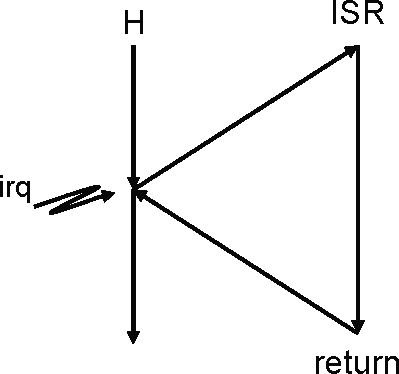
\includegraphics[scale=\figscale]{images/intsimpleinterruptdispatch}
%\caption{Eenvoudige voorstelling van een interruptafhandeling.}
%\label{fig:intsimpleinterruptdispatch}
%\end{figure}

\begin{figure}[!ht]
\centering
\begin{tikzpicture}[line width=1pt,font=\sffamily\footnotesize,-latex,scale=0.80]
\draw (0,0)  node (H) [above] {H}  -- (0,-2) node (irq) [left] {irq \rotatebox[origin=c]{150}{\Large\Lightning}};
\draw (0,-2) -- (3,0) node[above] {ISR};
\draw (3,0)  -- (3,-4) node[below] {return};
\draw (3,-4) -- (0,-2);
\draw (0,-2) -- (0,-4);
\end{tikzpicture}
\caption{Eenvoudige voorstelling van een interruptafhandeling.}
\label{fig:intsimpleinterruptdispatch}
\end{figure}

ISR's lijken veel op gewone subroutines, maar er zijn verschillen:

\begin{itemize}
\item Een ISR wordt gestart door een interrupt, niet door een
instructie\footnote{Er zijn processoren die instructies hebben die
software-interrupts genereren, zoals de Intel x86-familie.}.

\item Direct nadat de interrupt is herkend, wordt de Global Interrupt Enable
vlag (de I-vlag) in het Status Register op 0 gezet. Dit zorgt ervoor dat de
ISR niet kan worden onderbroken door een (nieuwe) interruptaanvraag.

\item Voor terugkeer moet de instructie \lstinline|reti| (Return From
Interrupt) gebruikt worden. Deze instructie zet de Global Interrupt Enable
vlag weer aan.
\end{itemize}

Interrupts en subroutines hebben wel \'e\'en overeenkomst: in beide gevallen
wordt de program counter (PC) op de stack gezet. Dit wordt uitgebeeld in
figuur~\ref{fig:intinterruptdispatchwithstackandiflag}. Omdat het
terugkeeradres op de stack wordt gezet, moet de stack pointer (SP) worden
ge\"initialiseerd v\'o\'ordat de interrupts mogen worden afgehandeld. Dat
betekent dat direct na het starten van het lopende programma, bijvoorbeeld
na een reset, de interrupts afgeschakeld zijn omdat de
stack pointer nog niet is ge\"initialiseerd.

%\begin{figure}[!ht]
%\centering
%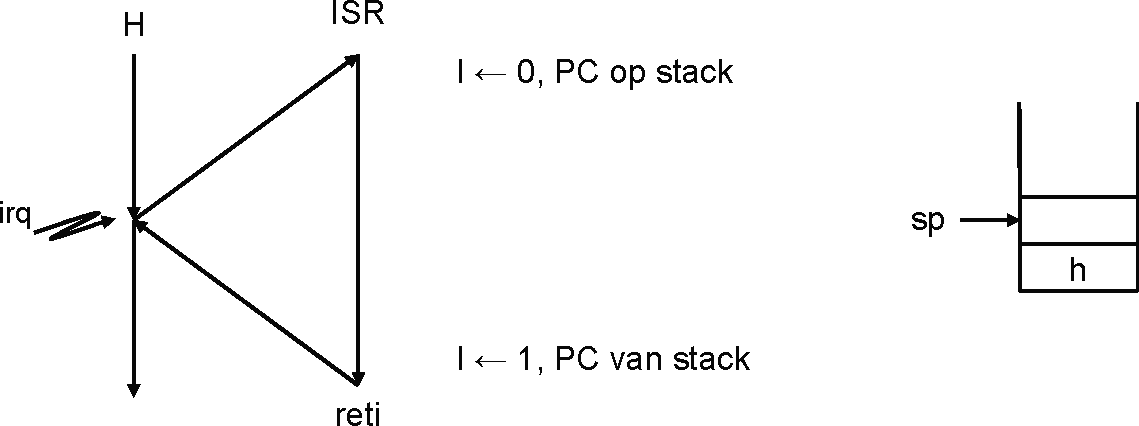
\includegraphics[scale=\figscale]{images/intinterruptdispatchwithstackandiflag}
%\caption{Interruptafhandeling: de program counter wordt op de stack gezet.}
%\label{fig:intinterruptdispatchwithstackandiflag}
%\end{figure}

\begin{figure}[!ht]
\centering
\begin{tikzpicture}[line width=1pt,font=\sffamily\footnotesize,-latex,scale=0.80]
\draw (0,0)  node (H) [above] {H}  -- (0,-2) node (irq) [left] {irq \rotatebox[origin=c]{150}{\Lightning}};
\draw (0,-2) -- (3,0) node[above] {ISR} node [right, xshift=.5cm] {I $\leftarrow$ 0, PC op stack};
\draw (3,0)  -- (3,-4) node[below] {reti} node [right, xshift=.5cm] {I $\leftarrow$ 1, PC van stack};
\draw (3,-4) -- (0,-2);
\draw (0,-2) -- (0,-4);
\draw[-] (11,-1) -- ++(0,-1)
         rectangle node[xshift=-1.4cm] {sp $\longrightarrow$} ++(1.5,-0.5)
         rectangle ++(-1.5,-0.5) node[pos=.5] {h}
++(1.5,1) -- ++(0,1);
\end{tikzpicture}
\caption{Interruptafhandeling: de program counter wordt op de stack gezet.}
\label{fig:intinterruptdispatchwithstackandiflag}
\end{figure}

Twee instructies be\"invloeden direct de I-flag:

\qquad \lstinline|sei| - set Global Interrupt Enable flag, interrupts worden
afgehandeld.

\qquad\lstinline|cli| - clear Global Interrupt Enable flag, interrupts worden
geblokkeerd.

De I-vlag is gepositioneerd op bit 7 van het Status Register (SREG). Zie
figuur~\ref{fig:intsregregisterlayout}. Het Status Register is in het I/O-geheugen
te vinden op adres 0x3f.

%%%% SREG
\begin{registerdef}{Het Status Register SREG}{fig:intsregregisterlayout}
7 & 6 & 5 & 4 & 3 & 2 & 1 & 0 \\
\hline
\multicolumn{1}{|c}{I} & \multicolumn{1}{|c}{T} & \multicolumn{1}{|c}{H} & \multicolumn{1}{|c}{S} & \multicolumn{1}{|c}{V} & \multicolumn{1}{|c}{N} & \multicolumn{1}{|c}{Z} & \multicolumn{1}{|c|}{C} \\ \hline
R/W & R/W & R/W & R/W & R/W & R/W & R/W & R/W \\
0 & 0 & 0 & 0 & 0 & 0 & 0 & 0 \\
\end{registerdef}
%%%% SREG

Pas na het initialiseren van de stack pointer mag de instructie
\lstinline|sei| gegeven worden.


\section{Interruptbronnen}
De ATmega32 kent veel interruptbronnen. Zo kan de ATmega32 reageren op
drie externe interrupts: INT0, INT1 en INT2. Verder kan de analoog-digitaal
converter (ADC) een interrupt geven als de conversie klaar is. De seri\"ele
interface (USART) kent naast een interrupt wanneer een karakter is ontvangen
ook een interrupt voor wanneer een karakter is verzonden. De nog te bespreken
timer/counters (zie hoofdstuk~\ref{cha:timercounters}) kunnen een interrupt
afgeven wanneer een timer/counter ``over de kop'' gaat, dus wanneer een
timer/counter van de hoogste stand naar de laagste stand gaat. Verder zijn
er nog interrupts mogelijk van de EEPROM, de TWI- en de SPI-interface.

Al deze interruptbronnen hebben een eigen interrupt-enable-bit. Om een
interrupt van een bron ook daadwerkelijk te laten plaatsvinden, moet deze
bit geactiveerd zijn (logisch~1) \'en de I-vlag moet logisch 1 zijn.

De ATmega32 heeft geen \textsl{software interrupts}. Dat zijn
software-instructies die interrupts genereren. Deze zijn wel na te bootsen
met INT0, INT1 en INT2.


\section{De Interrupt Vector Table}
We hebben nu besproken hoe het verwerken van een interrupt wordt uitgevoerd.
Maar nu rijst de vraag: waar moet de ISR beginnen? We zouden hiervoor een
vast adres in de Flash-ROM kunnen kiezen, bijvoorbeeld adres 0x1000.
Vervolgens reserveren we 512 bytes voor de ISR. De volgende ISR begint dan
op adres 0x1200. Hoewel dit natuurlijk te realiseren is, kleven hier wel
wat nadelen aan. Ten eerste moet de ISR altijd op adres 0x1000 beginnen.
Ten tweede kan de ISR niet groter zijn dan 512 bytes. Als de ISR korter is
dan 512 bytes, dan gebruiken we een gedeelte van de Flash-ROM niet (bedenk
dat de volgende ISR op adres 0x1200 begint). Ten derde moet de Flash-ROM
minimaal 4608 (= 0x1200) bytes groot zijn. We zien nu dat een vast adres
en een vaste lengte voor een ISR niet flexibel is.

We kunnen deze drie problemen oplossen door gebruik te maken van een
\textsl{Interrupt Vector Table}. Dit werkt als volgt. Aan elke interrupt is
een zogenoemde \textsl{Interrupt Vector} gekoppeld. Dit is een vast adres
in de Flash-ROM waar naartoe gesprongen wordt als een interrupt is herkend.
Elke vector is twee words (vier bytes) groot. Na het herkennen van de
interrupt wordt de PC dus geladen met het adres van de Interrupt Vector die
bij de interrupt hoort.
Aangezien elke Interrupt Vector slechts twee words groot is, zal op die
plek een spronginstructie naar de eigenlijke ISR geplaatst worden. Het
uitvoeren gebeurt dus in twee stappen: eerst naar de Interrupt Vector
springen en van daaruit naar de eigenlijk ISR. Het gebruik van de
Interrupt Vector Table is weergegeven in
figuur~\ref{fig:intinterruptdispatchwithvectortable}.

%\begin{figure}[!ht]
%\centering
%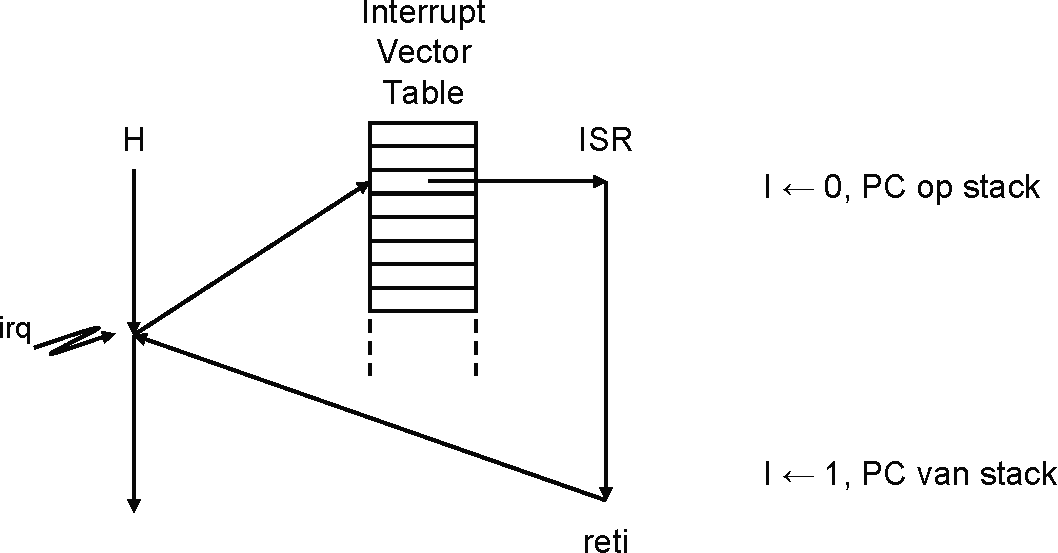
\includegraphics[scale=\figscale]{images/intinterruptdispatchwithvectortable}
%\caption{Interruptafhandeling: gebruik van de Interrupt Vector Table.}
%\label{fig:intinterruptdispatchwithvectortable}
%\end{figure}

\begin{figure}[!ht]
\centering
\begin{tikzpicture}[line width=1pt,font=\sffamily\footnotesize,-latex,scale=0.80]
\draw (0,0)  node (H) [above] {H}  -- (0,-2) node (irq) [left] {irq \rotatebox[origin=c]{150}{\Lightning}};
\draw (3,0) rectangle ++(1.5,-0.4) node[above,pos=0.5,yshift=2mm,align=center] {Interrupt\\Vector\\Table}
            rectangle ++(-1.5,-0.4)
            rectangle ++(1.5,-0.4) node[pos=0.5] (A) {}
			rectangle ++(-1.5,-0.4)
               --     ++(0,-1)
  ++(1.5,1)    --     ++(0,-1);
\draw (0,-2) -- (3,-1);
\draw (0,-2) -- (0,-4);
\draw (A) -- (7,-1) node [above] {ISR} node [right, xshift=.5cm] {I $\leftarrow$ 0, PC op stack};
\draw (7,-1) -- (7,-4) node[below] {reti} node [right, xshift=.5cm] {I $\leftarrow$ 1, PC van stack};
\draw (7,-4) -- (0,-2);
\end{tikzpicture}
\caption{Interruptafhandeling: gebruik van de Interrupt Vector Table.}
\label{fig:intinterruptdispatchwithvectortable}
\end{figure}

De Interrupt Vector Table ligt aan het begin van de Flash-ROM, van adres
0x000 t/m 0x029. Dat betekent dat de eerste vrije plaats 0x02a is. Vanaf
hier kan het gebruikersprogramma geplaatst worden. Na een reset is de PC
geladen met 0x000, dus wordt de instructieverwerking begonnen bij de eerste
vector. Deze is dan ook gereserveerd voor de Reset Vector. Op de Reset Vector
wordt dan een spronginstructie naar adres 0x02a geplaatst.

Natuurlijk heeft het gebruik van de Interrupt Vector Table een keerzijde.
Zo zijn er extra geheugenplaatsen nodig voor het opslaan van de vectoren.
De executietijd van de interrupt (Engels: interrupt latency) wordt met
drie klokpulsen verhoogd omdat er een sponginstructie moet worden uitgevoerd.

Een overzicht van de Interrupt Vector Table is te vinden in
tabel~\ref{tab:intinterruptvectortable}. Op adres 0x000 is de Reset Vector
geplaatst. Daarna volgt op adres 0x002 de vector voor de eerste externe
interrupt, dan voor de tweede externe interrupt, enzovoorts.

\begin{table}[!ht]
\centering
\caption{Interruptvectortabel voor de ATmega32.}
\label{tab:intinterruptvectortable}
\setlength{\tabcolsep}{8pt}
\begin{tabu}{ccll}
\toprule
vector \# & ROM-adres & Bron          & Omschrijving \\ \midrule
 1        & 0x000     & RESET         & Reset vector \\
 2        & 0x002     & INT0          & External Interrupt request 0 \\
 3        & 0x004     & INT1          & External Interrupt request 1 \\
 4        & 0x006     & INT2          & External Interrupt request 2 \\
 5        & 0x008     & TIMER2\_COMP  & Timer/Counter2 Compare Match \\
 6        & 0x00A     & TIMER2\_OVF   & Timer/Counter2 Overflow \\
 7        & 0x00C     & TIMER1\_CAPT  & Timer/Counter1 Capture Event \\
 8        & 0x00E     & TIMER1\_COMPA & Timer/Counter1 Compare Match A \\
 9        & 0x010     & TIMER1\_COMPB & Timer/Counter1 Compare Match B \\
10        & 0x012     & TIMER1\_OVF   & Timer/Counter1 Overflow \\
11        & 0x014     & TIMER0\_COMP  & Timer/Counter0 Compare Match \\
12        & 0x016     & TIMER0\_OVF   & Timer/Counter0 Overflow \\
13        & 0x018     & SPI, STC      & Serial Transfer Complete \\
14        & 0x01A     & USART, RXC    & USART, Rx Complete \\
15        & 0x01C     & USART, UDRE   & USART Data Register Empty \\
16        & 0x01E     & USART, TXC    & USART, Tx Complete \\
17        & 0x020     & ADC           & ADC Conversion Complete \\
18        & 0x022     & EE\_RDY       & EEPROM Ready \\
19        & 0x024     & ANA\_COMP     & Analog Comparator \\
20        & 0x026     & TWI           & Two-wire Serial Interface \\
21        & 0x028     & SPM\_RDY      & Store Program Memory Ready \\
\bottomrule
\end{tabu}
\raggedright\footnotesize Noot: het ROM-adres is in words.
\end{table}


\section{Interruptpriotiteit}
Als twee interrupt tegelijk binnenkomen, wordt de interrupt met de laagste
Interrupt Vector als eerste uitgevoerd. Er zijn dus prioriteiten aan de
interrupts gekoppeld. De interrupt die op dat moment niet wordt uitgevoerd,
moet wachten totdat de uitgevoerde interrupt afgehandeld is. Komt er echter
in de tussentijd een interrupt binnen met een lagere Interrupt Vector
dan wordt die weer als eerste uitgevoerd.


\section{Interruptresponstijd}
De responstijd voor alle ingeschakelde interrupts van de ATmega32 is minimaal
vier klokcycli. Tijdens deze vier klokcycli wordt de program counter op de
stack geplaatst (twee bytes) en wordt de program counter geladen met het
vectoradres van de interrupt. Na vier klokcycli wordt gesprongen naar het
vectoradres van de interrupt die wordt verwerkt. De instructie op de vector
is normaal gesproken een sprong naar de interruptroutine en deze sprong duurt
drie klokcycli voor een \lstinline|jmp|-instructie en twee klokcycli voor een
\lstinline|rjmp|-instructie.

Als een interrupt optreedt tijdens de uitvoering van een instructie met
meerdere klokcycli dan wordt deze instructie afgemaakt voordat de interrupt
wordt verwerkt. Staat de ATmega32 in slaapstand dan wordt de responstijd met
vier klokcycli verhoogd. Deze verhoging komt bovenop de opstarttijd van de
geselecteerde slaapmodus.

Een terugkeer (return) uit een interruptroutine duurt vier klokcycli. Tijdens
deze vier klokcycli wordt de program counter van de stack gehaald (twee bytes)
en wordt de stack pointer met twee verhoogd. Tevens wordt de I-bit in het
statusregister op 1 gezet.


\section{Stappen in de interruptverwerking}
Als een interruptsignaal bij de processor binnenkomt, worden de volgende
stappen genomen:
\begin{enumerate}
\item De processor maakt de instructie af die op dat moment wordt uitgevoerd.
      Dit is een instructie in het lopende programma.
\item De processor slaat het adres van de volgende instructie op de stack op.
      Dit adres staat in de program counter. De Global Interrupt Enable vlag
      wordt op 0 gezet.
\item De processor springt naar de interrupt vector. Dit is een vaste
      geheugenlocatie in de Flash-ROM.
\item Vanuit de interrupt vector wordt gesprongen naar het adres van de
      daadwerkelijke ISR.
\item Bij terugkeer uit de ISR wordt de program counter geladen met het adres
      dat op de stack gezet was. De Global Interrupt Enable vlag wordt op 1
      gezet.
\item De processor vervolgt het uitvoeren van het programma. Er wordt altijd
      \'e\'en instructie uitgevoerd voordat een eventuele nieuwe interrupt
      wordt verwerkt.
\end{enumerate}


\section{Algemene opzet interruptafhandeling}
In listing~\ref{cod:intgenericsetup} is de algemene opzet te zien voor een
programma met een interrupt. In regel 3 wordt het ROM-adres op 0x000 gezet.
Dat is de plek van de reset-vector. Op die plek wordt een spronginstructie
naar het begin van het eigenlijke programma gezet. In regel 7 wordt het
ROM-adres op het adres van de interruptvector gezet. We kunnen dit adres
vinden in tabel~\ref{tab:intinterruptvectortable}. Ook hier wordt een
spronginstructie gezet, nu naar het begin van de ISR (regel 9).

Nadat alle interruptvectoren voorzien zijn van spronginstructies, volgt de
code voor het initialiseren van de stack pointer. Dit is te zien in de
regels~15 t/m~18. Daarna volgen de instructies die de interruptbron nog
specifiek instellen. Te denken valt aan flankgevoeligheid van het interruptsignaal.
Deze specifieke instellingen worden in I/O-registers ingesteld.

Als alle instellingen zijn gedaan, worden de interrupt vrijgegeven door middel
van een \lstinline|sei|-instructie (regel 24). Daarna volgt het hoofdprogramma.
Dit is meestal een eeuwig durende lus (regels 27 t/m 29). Daarna worden de
instructies van de ISR geplaatst. Dat hoeft niet per se na de hoofdprogrammalus,
maar dat wordt wel vaak gedaan. De ISR eindigt met een \lstinline|reti|-instructie
(regel 34).

\begin{figure}[!t]
\begin{lstlisting}[language=AVRassembler,caption=Algemene opzet voor gebruik van interrupts.,label=cod:intgenericsetup]
.def temp = r16

.org 0x000
        ; reset vector
		rjmp reset

.org <address in vector table>
        ; ISR vector for ...
		rjmp isr

.org 0x02a
        ; Program starts here
reset:
		; set up stack pointer
		ldi	 temp,low(RAMEND)
		out	 SPL,temp
		ldi	 temp,high(RAMEND)
		out	 SPH,temp
		
        ; Specific set up for interrupt
        ...

		; enable interrupts
		sei

		; main program loop
loop:   ...
        ...
        rjmp loop

isr:    ; ISR code
        ...
        ...
 		reti
\end{lstlisting}
\end{figure}


\section{Context switch}
\label{sec:contextswitch}
Een interrupt kan op elk willekeurig moment plaatsvinden. We noemen zulke
interrupts \textsl{asynchroon}. Asynchroon houdt in dat het moment van
de interrupt niet (helemaal) te voorspellen is\footnote{Interrupts van
bijvoorbeeld de timer/counters zijn natuurlijk wel uit te rekenen.}. Stel
dat het lopende programma een complexe berekening aan het uitvoeren is.
De berekening zorgt ervoor dat de vlaggen en de registers worden aangepast.
Als nu een interrupt binnenkomt en de ISR wordt gestart dan is er een
grote kans dat in de ISR ook registers en de vlaggen worden aangepast.
Bij terugkeer naar het lopende programma moeten dan de originele waarden
van de registers en de vlaggen weer beschikbaar zijn om de berekening
correct te laten verlopen, d.w.z.\@ dat de \textsl{context} weer hersteld
moet worden. Het is daarom belangrijk om in de ISR de gebruikte registers
en de vlaggen op te slaan. Dat kan door gebruik te maken van de stack. 

In listing~\ref{cod:intcontextswich} is te zien hoe de vlaggen op de stack
geplaatst worden. De vlaggen zijn op te vragen via I/O-register
\lstinline|SREG|. Nu kan de inhoud van een I/O-register niet direct op de
stack geplaatst worden. Dit moet via een register. Dat betekent dat de inhoud
van dat register eerst op de stack geplaatst moet worden. Daarna worden de
vlaggen ingelezen in het register en op de stack gezet.

\begin{figure}[!ht]
\begin{lstlisting}[language=AVRassembler,caption=Opslaan van de registers en vlaggen.,label=cod:intcontextswich]
ISR:	push r16		; push R16
		in   r16,SREG	; SREG in I/O memory ...
		push r16		; ... so push flags via R16
		
		; rest of the ISR code

		pop  r16		; pop flags via R16
		out  SREG,r16
		pop  r16		; pop R16
		reti			; return
\end{lstlisting}
\end{figure}

Aan het einde van de ISR moeten de registers en de vlaggen weer van de stack
gehaald worden. Let daarbij op de volgorde van de registers.


\section{Externe interrupts}
De ATmega32 kent drie externe interrupts genaamd INT0, INT1 en INT2. Deze
interrupts zijn fysiek verbonden met Port~D, bit~2 (PD2, INT0), Port~D, bit~3
(PD3, INT1) en Port~B, bit~2 (PB2, INT2). INT0 en INT1 kunnen zowel op een
laag niveau als op flanken reageren. INT2 kan alleen op flanken reageren.
Zoals te
zien in tabel~\ref{tab:intinterruptvectortable} worden de vectoradressen
0x002, 0x004 en 0x006 gebruikt voor respectievelijk INT0, INT1, en INT2. We
merken op dat INT0 dus een hogere prioriteit heeft dan INT1 en INT2.

Om een externe interrupt te herkennen, moeten de bijbehorende pinnen als
ingang gedefinieerd worden. Maar er moet opgemerkt worden dat interrupts
ook worden herkend als de bijbehorende pin als uitgang gedefinieerd is. Op
deze manier is het mogelijk om vanuit de software een interrupt te genereren. 

Het General Interrupt Control Register (GICR) heeft drie bits waarmee de INT’s
kunnen worden geactiveerd. Een logische 1 in de betreffende bit activeert de
INT. Merk op dat de I-vlag in het Status Reister 1 moet zijn om interrupt ook
daadwerkelijk te laten plaatsvinden. De indeling van het GICR is te vinden in
figuur~\ref{fig:intgicr}. Alleen de bits 5, 6 en~7 zijn van belang. 

%%%% GICR
\begin{registerdef}{Het GICR register}{fig:intgicr}
7 & 6 & 5 & 4 & 3 & 2 & 1 & 0 \\
\hline
\multicolumn{1}{|c}{INT1} & \multicolumn{1}{|c}{INT0} & \multicolumn{1}{|c}{INT2} & \multicolumn{1}{|c}{\cellcolor{regcell} $-$} & \multicolumn{1}{|c}{\cellcolor{regcell} $-$} & \multicolumn{1}{|c}{\cellcolor{regcell} $-$} & \multicolumn{1}{|c}{\cellcolor{regcell} IVSEL} & \multicolumn{1}{|c|}{\cellcolor{regcell} IVCE} \\ \hline
R/W & R/W & R/W & R & R & R & R/W & R/W \\
0 & 0 & 0 & 0 & 0 & 0 & 0 & 0 \\
\end{registerdef}
%%%% GICR

In listing~\ref{cod:intenableint0} is te zien hoe INT0 geactiveerd wordt.
Merk op dat de betreffende bit in het Data Direction Register D (DDRD, bit 2)
op 0 moet staan om de pin als ingang te defini\"eren.

\begin{figure}[!ht]
\begin{lstlisting}[language=AVRassembler,caption=Het activeren van INT0.,label=cod:intenableint0]
    ldi r16,0b01000000  ; activate INT0 (pin PD2)
    out GICR,r16
\end{lstlisting}
\end{figure}

Een flankgevoelige interrupt (opgaande flank, neergaande flank of beide
flanken) wordt door de ATmega32 ``ingevangen''. Dit wordt bijgehouden in
het General Interrupt Flag Register (GIFR). Dat betekent dat als een
flankgevoelige interrupt wordt herkend, de bijbehorende bit in het
GIFR-register op 1 wordt gezet. Als de ISR wordt uitgevoerd, wordt de
bit door de hardware op 0 gezet. Zolang een interruptaanvraag niet
wordt uitgevoerd blijft de bit dus 1. In figuur~\ref{fig:intgifr} is
de indeling van het GIFR-register te zien. Merk op dat een niveaugevoelige
interrupt (INT0, INT1) de bijbehorende bits in het GIFR-register niet op
1 zet. Bij niveaugevoelige interrupts wordt direct de status van de pinnen
ingelezen.

%%%% GIFR
\begin{registerdef}{Het GIFR register}{fig:intgifr}
7 & 6 & 5 & 4 & 3 & 2 & 1 & 0 \\
\hline
\multicolumn{1}{|c}{INTF1} & \multicolumn{1}{|c}{INTF0} & \multicolumn{1}{|c}{INTF2} & \multicolumn{1}{|c}{\cellcolor{regcell} $-$} & \multicolumn{1}{|c}{\cellcolor{regcell} $-$} & \multicolumn{1}{|c}{\cellcolor{regcell} $-$} & \multicolumn{1}{|c}{\cellcolor{regcell} $-$} & \multicolumn{1}{|c|}{\cellcolor{regcell} $-$} \\ \hline
R/W & R/W & R/W & R & R & R & R & R \\
0 & 0 & 0 & 0 & 0 & 0 & 0 & 0 \\

\end{registerdef}
%%%% GIFR

Merk op dat een bit in het GIFR-register door software op 0 kan worden gezet
door er een 1 naar toe te schrijven. Dit principe geldt voor alle interrupts
die de ATmega32 kent.

\subsubsection*{Triggermogelijkheden van INT0 en INT1}
Zowel INT0 als INT1 kunnen op meerdere mogelijkheden geactiveerd worden.
Ze kunnen reageren op een laag niveau, op een opgaande flank, op een
neergaande flank of op beide flanken. Ze kunnen niet reageren op een
hoog niveau. De mogelijkheden worden aangegeven met de ISC-bits in het
MCU Control Register (MCUCR). De indeling van dit register is te zien
in figuur~\ref{fig:intmcucr}. 

%%%% MCUCR
\begin{registerdef}{Het MCUCR register}{fig:intmcucr}
7 & 6 & 5 & 4 & 3 & 2 & 1 & 0 \\
\hline
\multicolumn{1}{|c}{\cellcolor{regcell} SE} & \multicolumn{1}{|c}{\cellcolor{regcell} SM2} & \multicolumn{1}{|c}{\cellcolor{regcell} SM1} & \multicolumn{1}{|c}{\cellcolor{regcell} SM0} & \multicolumn{1}{|c}{ISC11} & \multicolumn{1}{|c}{ISC10} & \multicolumn{1}{|c}{ISC01} & \multicolumn{1}{|c|}{ISC00} \\ \hline
R/W & R/W & R/W & R/W & R/W & R/W & R/W & R/W \\
0 & 0 & 0 & 0 & 0 & 0 & 0 & 0 \\
\end{registerdef}
%%%% MCUCR

\textbf{Bit 3, 2 – ISC11, ISC10: Interrupt Sense Control 1 bit 1 en bit 0} \\
De ISC11- en ISC10-bits defini\"eren de wijze waarop INT1 een interrupt
genereert. De INT1-pin (PD3) wordt bemonsterd voordat de flank wordt
gedetecteerd. Als flankgevoelige triggering is geselecteerd, worden pulsen
groter dan \'e\'en klokcyclus herkend. Als een puls korter is dan \'e\'en
klokcyclus dan is er geen garantie dat de puls (en dus de flank) wordt
herkend. Als triggering van een laag niveau wordt gebruikt, dan moet het
lage niveau aangehouden worden totdat de huidige instructie uitgevoerd is.
De langstdurende instructie is een \lstinline|call|-instructie. Deze
instructie duurt op een ATmega32 vier klokcycli. Dat betekent dat het
lage niveau op de INT1-pin dus minimaal vier klokcycli moet duren. De
interrupt wordt (steeds) herkend zolang het lage niveau aangehouden wordt.
In figuur~\ref{tab:inttriggerint1} is te zien hoe een bepaalde triggering
ingesteld moet worden.

\begin{table}[!ht]
\centering
\caption{Triggermogelijkheden van INT1.}
\label{tab:inttriggerint1}
\setlength{\tabcolsep}{8pt}
\begin{tabular}  {>{\centering\arraybackslash}m{1cm}>{\centering\arraybackslash}m{1cm}>{\centering\arraybackslash}m{2cm}m{7cm}}
\toprule
ISC11 & ISC10 & & Omschrijving \\ \midrule
  0   &   0   & \begin{tikzpicture}\draw (0,0.3) -- (0.3,0.3) -- (0.3,0);\draw [ultra thick] (0.3,0.0) -- (1.3,0);\draw (1.3,0) -- (1.3,0.3) -- (1.6,0.3);\end{tikzpicture} & Een laag niveau op de INT1-ingang genereert een interrupt. \\ \midrule
  0   &   1   & \begin{tikzpicture}\draw (0,0.3) -- (0.3,0.3);\draw [ultra thick] (0.3,0.3) -- (0.3,0.0);\draw (0.3,0) -- (1.3,0);\draw [ultra thick] (1.3,0) -- (1.3,0.3);\draw (1.3,0.3) -- (1.6,0.3);\end{tikzpicture} & Een opgaande en neergaande flank op de INT1-ingang genereert een interrupt. \\ \midrule
  1   &   0   & \begin{tikzpicture}\draw (0,0.3) -- (0.3,0.3);\draw [ultra thick] (0.3,0.3) -- (0.3,0.0);\draw (0.3,0) -- (1.3,0);\draw (1.3,0) -- (1.3,0.3);\draw (1.3,0.3) -- (1.6,0.3);\end{tikzpicture} & Een neergaande flank op de INT1-ingang genereert een interrupt. \\ \midrule
  1   &   1   & \begin{tikzpicture}\draw (0,0.3) -- (0.3,0.3);\draw (0.3,0.3) -- (0.3,0.0);\draw (0.3,0) -- (1.3,0);\draw [ultra thick] (1.3,0) -- (1.3,0.3);\draw (1.3,0.3) -- (1.6,0.3);\end{tikzpicture} & Een opgaande flank op de INT1-ingang genereert een interrupt. \\
\bottomrule
\end{tabular}
\end{table}

In listing~\ref{cod:intenablerisingedgeint1} is te zien hoe INT1 wordt
ingesteld voor het herkennen van een opgaande flank om een interrupt te
genereren.

\begin{figure}[!ht]
\begin{lstlisting}[language=AVRassembler,caption=Instellen van de opgaande  flank voor INT11.,label=cod:intenablerisingedgeint1]
    ldi r16,0b00001100  ; activate rising edge INT1
    out MCUCR,r16
\end{lstlisting}
\end{figure}

\textbf{Bit 1, 0 – ISC01, ISC00: Interrupt Sense Control 0 bit 1 en bit 0} \\
De ISC01- en ISC00-bits defini\"eren de wijze waarop INT0 een interrupt
genereert. De werking is identiek aan die van de ISC-bits van INT1. Ook de
timing is identiek. Zie tabel~\ref{tab:inttriggerint0}.

\begin{table}[!ht]
\centering
\caption{Triggermogelijkheden van INT0.}
\label{tab:inttriggerint0}
\setlength{\tabcolsep}{8pt}
\begin{tabular}  {>{\centering\arraybackslash}m{1cm}>{\centering\arraybackslash}m{1cm}>{\centering\arraybackslash}m{2cm}m{7cm}}
\toprule
ISC01 & ISC00 & & Omschrijving \\ \midrule
  0   &   0   & \begin{tikzpicture}\draw (0,0.3) -- (0.3,0.3) -- (0.3,0);\draw [ultra thick] (0.3,0.0) -- (1.3,0);\draw (1.3,0) -- (1.3,0.3) -- (1.6,0.3);\end{tikzpicture} & Een laag niveau op de INT0-ingang genereert een interrupt. \\ \midrule
  0   &   1   & \begin{tikzpicture}\draw (0,0.3) -- (0.3,0.3);\draw [ultra thick] (0.3,0.3) -- (0.3,0.0);\draw (0.3,0) -- (1.3,0);\draw [ultra thick] (1.3,0) -- (1.3,0.3);\draw (1.3,0.3) -- (1.6,0.3);\end{tikzpicture} & Een opgaande en neergaande flank op de INT0-ingang genereert een interrupt. \\ \midrule
  1   &   0   & \begin{tikzpicture}\draw (0,0.3) -- (0.3,0.3);\draw [ultra thick] (0.3,0.3) -- (0.3,0.0);\draw (0.3,0) -- (1.3,0);\draw (1.3,0) -- (1.3,0.3);\draw (1.3,0.3) -- (1.6,0.3);\end{tikzpicture} & Een neergaande flank op de INT0-ingang genereert een interrupt. \\ \midrule
  1   &   1   & \begin{tikzpicture}\draw (0,0.3) -- (0.3,0.3);\draw (0.3,0.3) -- (0.3,0.0);\draw (0.3,0) -- (1.3,0);\draw [ultra thick] (1.3,0) -- (1.3,0.3);\draw (1.3,0.3) -- (1.6,0.3);\end{tikzpicture} & Een opgaande flank op de INT0-ingang genereert een interrupt. \\
\bottomrule
\end{tabular}
\end{table}

\subsubsection*{Triggermogelijkheden van INT2}
Externe interrupt INT2 kan alleen op de opgaande flank of op de neergaande
flank triggeren. Dit is in te stellen in het MCU Control and Status Register
(MCUCSR). De indeling van dit register is te zien in
figuur~\ref{fig:intmcucsr}. INT2 wordt \textsl{asynchroon} verwerkt.
Asynchroon betekent hier dat het interruptsignaal buiten de klok om wordt
``ingevangen''. De minimale pulsduur van INT2 is 50 ns, maar de puls wordt
dus niet bemonsterd op klokflanken van de systeemklok. De aanvraag wordt
wel verwerkt op de flanken van de systeemklok.

%%%% MCUCSR
\begin{registerdef}{Het MCUCSR register}{fig:intmcucsr}
7 & 6 & 5 & 4 & 3 & 2 & 1 & 0 \\
\hline
\multicolumn{1}{|c}{\cellcolor{regcell} JTD} & \multicolumn{1}{|c}{ISC2} & \multicolumn{1}{|c}{\cellcolor{regcell} $-$} & \multicolumn{1}{|c}{\cellcolor{regcell} JTRF} & \multicolumn{1}{|c}{\cellcolor{regcell} WDRF} & \multicolumn{1}{|c}{\cellcolor{regcell} BORF} & \multicolumn{1}{|c}{\cellcolor{regcell} EXTRF} & \multicolumn{1}{|c|}{\cellcolor{regcell} PORF} \\ \hline
R/W & R/W & R & R/W & R/W & R/W & R/W & R/W \\
0 & 0 & 0 & 0 & 0 & 0 & 0 & 0 \\
\end{registerdef}
%%%% MCUCSR

\textbf{Bit 6 - ISC2: Interrupt Sense Control 2}\\
Bit ISC2 geeft aan op welke flank INT2 moet reageren. Een 0 geeft aan dat INT2
op een neergaande flank triggert, een 1 geeft aan dat INT2 op een opgaande
flank triggert.

Bij het wijzigen van de ISC2-bit kan een interrupt optreden. Daarom is het
nodig om INT2 eerst uit te schakelen door het uitschakelen van de INT2-bit
in het GICR-register. Vervolgens kan de ISC2-bit worden gewijzigd. Daarna
moet een eventuele interruptaanvraag worden gewist door een logische 1
naar de INTF2-bit in het GIFR-register te schrijven voordat de interrupt
opnieuw wordt ingeschakeld. In listing~\ref{cod:intexamplecodeint2} is te
zien hoe van flank kan worden gewisseld.

\begin{figure}[!ht]
\begin{lstlisting}[language=AVRassembler,caption=Omschakelen van INT2 van neergaande naar opgaande flank.,label=cod:intexamplecodeint2]
    ; Disable INT2, leave INT0/INT1 untouched
    in   r16,GICR
    andi r16,0b11011111
    out  GICR,r16
    
    ; Change falling edge to rising edge, don't touch other flags
    in   r16,MCUCSR
    ori  r16,0b01000000
    out  MCUCSR,r16
    
    ; Clear INTF2 flag
    ldi  r16,0x00100000
    out  GIFR,r16
    
    ; Enable INT2, leave INT0/INT1 untouched
    in   r16,GICR
    ori  r16,0b00100000
    out  GICR,r16
\end{lstlisting}
\end{figure}

In listing~\ref{cod:intexamplecodeint0} is een voorbeeld te zien van het
gebruik van INT0. Als taak heeft de ISR om de bits van Port B te
inverteren. We beginnen met het aangeven van de reset-vector (regel~5) en de
INT0-vector (regel~8). Daarna wordt de stack ge\"initialiseerd (regel~14
t/m~17). In regel~20 en~21 wordt Port B als uitgang ingesteld. In regel~24
en~25 wordt gekozen voor de opgaande flank van INT0. In regel~25 en~26
activeren we INT0. Daarna worden de interrupts vrij gegeven middels een
\lstinline|sei|-instructie (regel~32) en blijven we in een eeuwig durende lus
wachten (regel~35).

\begin{figure}[!p]
\begin{lstlisting}[language=AVRassembler,caption=Voorbeeldprogramma INT0 met opgaande flank en ISR.,label=cod:intexamplecodeint0]
.def temp = r16

.org 0x000
        ; reset vector
		rjmp reset
.org 0x002
        ; ISR vector for INT0
		rjmp int0_isr

.org 0x02a
        ; main program starts here
reset:
		; set up stack pointer
		ldi	 temp,low(RAMEND)
		out	 SPL,temp
		ldi	 temp,high(RAMEND)
		out	 SPH,temp
		
		; All pins Port B are outputs
		ldi  temp,0xff
		out  DDRB,temp

		; set up rising edge INT0
		ldi	 temp,0b00000011
		out	 MCUCR,temp

		; set up INT0
		ldi	 temp,0b01000000
		out	 GICR,temp

		; enable interrupts
		sei

		; forever....
loop: 	rjmp loop

int0_isr:
        ; save regs and flags
		push temp
		in   temp,SREG
		push temp

        ; Invert all Port B bits
        in   temp,PORTB
        com  temp
        out  PORTB,temp

		; restore regs and flags and return from interrupt
		pop	 temp
		out	 SREG,temp
		pop	 temp
 		reti
\end{lstlisting}
\end{figure}

In de ISR wordt de context (de processorstatus) op de stack gezet (regels~39
t/m~31). Daarna wordt Port B ingelezen, ge\"inverteerd en weer
teruggeschreven (regels~44 t/m~46). Vlak voor het terugkeren wordt de context
weer van de stack gehaald (regels~49 t/m~41). Daarna keren we weer terug naar
het lopende programma door middel van een \lstinline|reti|-instructie.

\section{Interrupts binnen interrupts}
Als een interrupt wordt afgehandeld, wordt de bijbehorende ISR gestart. Net
voordat ISR wordt gestart, wordt de Global Interrupt Enable vlag (I-vlag)
op~0 gezet. Dit zorgt ervoor dat nieuwe interruptaanvragen (nog) niet
afgehandeld worden. Deze aanvragen moeten wachten totdat de ISR klaar is.
Bij het terugkeren wordt de I-vlag weer op~1 gezet, zodat wachtende
interruptaanvragen kunnen worden afgehandeld.

Het is mogelijk om in een ISR de I-vlag weer op~1 te zetten zodat een
interruptaanvraag kan worden bediend. De ISR wordt dus onderbroken door
een interrupt en er wordt een (andere) ISR gestart. We spreken dan over
een interrupt binnen een interrupt.

Het kan handig zijn om een ISR te laten onderbreken door een interrupt.
Zo kan een ISR voor de afhandeling van een toetsaanslag prima onderbroken
worden door een interruptaanvraag van de netwerkkaart. We kunnen ongeveer
drie toetsaanslagen per seconden maken maar netwerkpakketten komen met
1 Gbps (gigabit per seconde) binnen. Het is dan belangrijk om deze
interrupt eerst af te handelen. Nadat de ISR van de netwerkkaart is
afgelopen, wordt weer verder gegaan met de ISR van het toetsenbord.

Voorzichtigheid is wel geboden met interrupts binnen interrupts, vooral
bij level-triggered interrupts. Zolang de logische waarde (level) wordt
aangehouden, wordt de ISR onderbroken door een interruptaanvraag. Daardoor
wordt elke keer als een ISR wordt gestart het terugkeeradres op de stack
gezet. De stack loopt zodoende snel vol wat resulteert in een \textsl{stack
overflow}.

\section{Software interrupts}
De ATmega32 kent geen instructies om een interrupt te genereren. Dit kan
echter wel nagebootst worden middels de externe interrupts zoals te zien
is in listing~\ref{cod:intint0swint}. In dit voorbeeld wordt INT0 gebruikt
voor het genereren van een interrupt. Dit kan gerealiseerd worden door
de externe interrupt pin PD2 (Port D, pin 2) als uitgang te defini\"eren.
Door het schrijven van een logische 1 naar PD2 wordt een opgaande flank
gerealiseerd die door de ATmega32 gezien wordt als een interruptaanvraag
voor INT0.

In de listing worden de vectoren en de stack ge\"initialiseerd (regels~1
t/m~10). In regel~12 en~13 wordt PD2 als uitgang gezet. In regels~15
t/m~19 wordt INT0 als flankgevoelige interrupt (opgaande flank) ingesteld.
Daarna worden de interrupts vrijgegeven. Om niet continu een interrupt te
genereren is een korte wachtlus ingebouwd. Die zorgt ervoor dat eens in
de~767 klokcycli een interrupt gegenereerd wordt. Eerst wordt PD2 op een
logische~0 gezet (regel~24). Daarna wordt de wachtlus gestart (regels~26
en~27). In regels~29 en~30 wordt PD2 logisch~1 gemaakt zodat een opgaande
flank wordt aangeboden aan de interrupthardware. Daarna wordt gesprongen
naar regel~23 zodat weer een logische~0 op PD2 gezet wordt en wordt de
wachtlus weer uitgevoerd.

\begin{figure}[!ht]
\begin{lstlisting}[language=AVRassembler,caption=Externe interrupt INT0 wordt gebruikt als software interrupt.,label=cod:intint0swint]
		.org 0x000
		rjmp start
		.org 0x002
		rjmp int0_isr

		.org 0x02a
start:	ldi  r16,low(RAMEND)   ; stack
		out  SPL,r16
		ldi  r16,high(RAMEND)
		out  SPH,r16

		ldi  r16,0b00000100    ; PD2 as output
		out  DDRD,r16

		ldi  r16,0b00000011    ; INT0 pos. edge
		out  MCUCR,r16

		ldi  r16,0b01000000    ; INT0 active
		out  GICR,r16

		sei                    ; free interrupts

again:	ldi  r16,0x00
        out  PORTD,r16         ; Port D2 off

delay:	subi r16,0x01          ; delay 767 clocks
		brne delay

		ldi  r16,0b00000100    ; generate interrupt
		out  PORTD,r16

		rjmp again

int0_isr:
		reti
\end{lstlisting}
\end{figure}

Software interrupt zijn in de ATmega32 niet echt nodig. Maar in de wereld
van de Operating Systems vormen ze een schakel tussen een gebruikersprogramma
en de \textsl{kernel}. Een gebruikersprogramma mag bijvoorbeeld niet zomaar
naar de harddisk schrijven maar moet deze acties via de kernel uitvoeren. Om
in \textsl{kernel mode} te komen, moet een software interrupt worden
uitgevoerd. De kernel bepaalt dan welke interrupt is aangevraagd en wat de te
verwachten actie is. Deze kernel routines worden \textsl{system calls} genoemd.
In programmeertalen zoals `C' zijn software interrupts niet direct te gebruiken.
In plaats daarvan zijn er functies zoals \lstinline|read| en \lstinline|write|
voorhanden. Een gebruikersprogramma voert bijvoorbeeld een \lstinline|read| uit
en in die functie wordt dan de software interrupt uitgevoerd.

\section{Interrupts in `C'}
De programmeertaal `C' is niet uitgerust om ISR's te programmeren. De GNU
AVR-C compiler heeft echter functies waarmee dit wel mogelijk is. Dit zijn dus
uitbreidingen op de taal `C' en kunnen niet gebruikt worden op bijvoorbeeld een
PC of een iMac.

Om gebruik te maken van de interruptfaciliteiten moet een header-bestand
geladen worden waarin functies zijn gedeclareerd. Dit is het bestand
\lstinline|avr/interrupt.h|. Aangezien de interrupts geactiveerd worden
via de I/O-registers moet ook \lstinline|avr/io.h| geladen worden. Dit is te
zien in listing~\ref{cod:intheaderfiles}. Het gebruik van header-bestand
\lstinline|avr/cpufunc.h| wordt verderop uitgelegd.

\begin{figure}[!ht]
\begin{lstlisting}[language=C,caption=Header-bestanden voor het gebruik van interrupts.,label=cod:intheaderfiles]
#include <avr/io.h>
#include <avr/interrupt.h>
#include <avr/cpufunc.h>
\end{lstlisting}
\end{figure}

Na het laden van header-bestand \lstinline|avr/interrupt.h| is voor het
coderen van een ISR de macro \lstinline|ISR(...)| beschikbaar. De definitie
van deze macro is complex en wordt verder niet besproken. Als argument aan
de macro moet in ieder geval de interruptvectornaam gegeven worden. Optioneel
kunnen enkele \textsl{atrributes} opgegeven worden.

%%\begin{figure}[!ht]
%%\begin{lstlisting}[language=C,caption=Header-bestanden voor het gebruik van interrupts.,label=cod:intheaderfiles]
%%ISR(vectornaam, attributes) { ... }
%%\end{lstlisting}
%%\end{figure}

In tabel~\ref{tab:intinterruptvectornames} zijn de interruptvectornamen te
zien. Deze namen moeten gebruikt worden bij de \lstinline|ISR|-macro.
Merk op dat de reset geen vectornaam heeft. Het is namelijk niet
mogelijk om een ISR voor de reset te coderen. De resetvector wordt
door de C-compiler ingevuld en zorgt ervoor dat, na initialisatie van
variabelen, de functie \lstinline|main()| wordt aangeroepen.

\begin{table}[!ht]
\centering
\caption{Interruptvectornamen voor ISR in `C' voor de ATmega32.}
\label{tab:intinterruptvectornames}
\setlength{\tabcolsep}{8pt}
\begin{tabu}{cll}
\toprule
vector \# & Bron          & Vectornaam \\ \midrule
 1        & RESET         & $-$ \\
 2        & INT0          & \lstinline|INT0_vect| \\
 3        & INT1          & \lstinline|INT1_vect| \\
 4        & INT2          & \lstinline|INT2_vect| \\
 5        & TIMER2\_COMP  & \lstinline|TIMER2_COMP_vect| \\
 6        & TIMER2\_OVF   & \lstinline|TIMER2_OVF_vect| \\
 7        & TIMER1\_CAPT  & \lstinline|TIMER1_CAPT_vect| \\
 8        & TIMER1\_COMPA & \lstinline|TIMER1_COMPA_vect| \\
 9        & TIMER1\_COMPB & \lstinline|TIMER1_COMPB_vect| \\
10        & TIMER1\_OVF   & \lstinline|TIMER1_OVF_vect| \\
11        & TIMER0\_COMP  & \lstinline|TIMER0_COMP_vect| \\
12        & TIMER0\_OVF   & \lstinline|TIMER0_OVF_vect| \\
13        & SPI, STC      & \lstinline|SPI_STC_vect| \\
14        & USART, RXC    & \lstinline|USART_RXC_vect| \\
15        & USART, UDRE   & \lstinline|USART_UDRE_vect| \\
16        & USART, TXC    & \lstinline|USART_TXC_vect| \\
17        & ADC           & \lstinline|ADC_vect| \\
18        & EE\_RDY       & \lstinline|EE_RDY_vect| \\
19        & ANA\_COMP     & \lstinline|ANA_COMP_vect| \\
20        & TWI           & \lstinline|TWI_vect| \\
21        & SPM\_RDY      & \lstinline|SPM_RDY_vect| \\
\bottomrule
\end{tabu}
\end{table}

In listing~\ref{cod:intisrforint0} is een compleet voorbeeld gegeven van het
gebruik van de INT0 ISR. De taak van de ISR is om pin PB0 (Port B, bit 0)
te laten toggelen. Na het laden van de header-bestanden wordt Port B
als uitgang gedefinieerd en wordt INT0
ge\"initialiseerd als een flankgevoelige interrupt op de opgaande flank
(regels 7 t/m 10). In regel 12 worden de interrupts vrijgegeven door het
aanzetten van de I-vlag middels het \lstinline|sei()|-statement. Daarna
wordt in een eeuwig durende lus gewacht middels het
\lstinline|while()|-statement.

\begin{figure}[!ht]
\begin{lstlisting}[language=C,caption=Voorbeeld van het gebruik van de INT0 interrupt service routine.,label=cod:intisrforint0]
#include <avr/io.h>
#include <avr/interrupt.h>
#include <avr/cpufunc.h>

int main(void) {
	
	DDRB  = 0xff;    /* Port B as output */
	
	MCUCR = 0x03;    /* INT0 rising edge */
	GICR  = 0x40;    /* INT0 active */
	
	sei();           /* Free interrupts */
	
    while (1) {
    }
}

ISR(INT0_vect) {     /* INT0 ISR */
	_NOP();          /* To set a breakpoint */
	PORTB ^= 0x01;   /* Flip PB0 */
	_NOP();          /* To set a breakpoint */
}
\end{lstlisting}
\end{figure}

Het \lstinline|sei()|-statement wordt vertaald naar een assembler
\lstinline|sei|-instructie. Er bestaat ook een \lstinline|cli()|-statement
dat vertaald wordt naar een assembler \lstinline|cli|-instructie.
In feite zijn dit macro's met de volgende definitie:

\begin{figure}[!ht]
\begin{lstlisting}[language=C,caption=Definitie van de sei()- en cli()-statements.,label=cod:intseiclidef]
#define sei()  __asm__ __volatile__ ("sei" ::: "memory")
#define cli()  __asm__ __volatile__ ("cli" ::: "memory")
\end{lstlisting}
\end{figure}

De constructie \lstinline|__asm__| signaleert aan de C-compiler dat wat
volgt een assemblerinstructie is. De constructie \lstinline|__volatile__|
geeft aan dat de C-compiler de assemblerinstructie letterlijk moet
overnemen en geen optimalisatie mag toepassen\footnote{De
\lstinline|sei|- en \lstinline|cli|-instructies passen geen
geheugenplaatsen en registers aan. De compiler zou hieruit de conclusie
kunnen trekken dat de beide instructies dus netto geen effect hebben en
dat ze dus verwijderd kunnen worden uit de gecompileerde code.}.

De ISR is gecodeerd in de regels 18 t/m 22 en heeft drie statements.
De macro \lstinline|_NOP()| in de regels 19 en 21 wordt vertaald
naar een assembler
\lstinline|nop|-instructie. Deze macro wordt gedefinieerd door het
header-bestand \lstinline|avr/cpufunc.h|. Het gebruik van deze macro
is handig bij het zetten van een breakpoint tijdens debuggen. Het
statement in regel 20 zorgt ervoor dat pin PB0 (Port B, bit 0) steeds
van waarde veranderd (toggelen). Het ``dakje''-teken \lstinline|^| 
(Nederland: accent circonflexe, Engels: circumflex) is de 
``C''-taalconstructie voor de EXOR-operatie. Het gehele statement
werkt als volgt. De waarde van \lstinline|PORTB| wordt gelezen,
de bits 1 t/m 7 wordt onveranderd overgenomen en bit 0 wordt
ge\"inverteerd. Daarna wordt de nieuwe waarde teruggeschreven naar
\lstinline|PORTB|.

\subsection{Bad Interrupt Handler}
Wat gebeurt er als een bepaalde interruptbron geactiveerd wordt maar er
is geen ISR beschikbaar, d.w.z.\@ er is geen ISR geprogrammeerd. Als
de betreffende interrupt geregistreerd wordt, zal de normale verwerking
van de interrupt plaatsvinden. Er wordt gesprongen naar het vectoradres
van de interrupt en daar wordt dan met de instructieverwerking begonnen.
Maar er is geen ISR beschikbaar dus kan er niet naar de ISR gesprongen
worden. De C-compiler lost dit op door alle niet gebruikte interrupts
om te leiden naar de zogenoemde Bad Interrupt Handler. Deze
\textsl{catch-all} ISR is als volgt in te stellen:

\begin{figure}[!ht]
\begin{lstlisting}[language=C,caption=De Bad Interrupt Handler.,label=cod:intbadisr]
#include <avr/interrupt.h>

ISR(BADISR_vect) {
	/* user code here */
}
\end{lstlisting}
\end{figure}

De standaard actie van de Bad Interrupt Handler is dat er naar de reset-vector
wordt gesprongen. Dit kan leiden tot een problematische uitvoering van het
programma. Het is daarom aan te bevelen om de Bad Interrupt Handler altijd
op te nemen in het programma. Merk op dat het ontbreken van een ISR duidt op
een programmeerfout.

\subsection{Interrupt prologue en epilogue}
In paragraaf~\ref{sec:contextswitch} is al beschreven dat tijdens het
uitvoeren van de ISR de gebruikte registers en de vlaggen op de stack
gezet moeten worden. De C-compiler zorgt hier automatisch voor. Dit wordt
de \textsl{prologue} van de ISR genoemd. Vlak voordat de ISR verlaten
wordt, worden de registers en de vlaggen weer van de stack gehaald.
Ook hier zorgt de C-compiler voor. Dit wordt de \textsl{epilogue}
genoemd. Merk op dat de C-compiler ook de \lstinline|reti|-instructie
automatisch toevoegt. 

\subsection{Naked interrupts}
Soms is het handig om de prologue en de epilogue niet door de C-compiler
te laten genereren, bijvoorbeeld als de interrupt met maximale snelheid
moet worden afgehandeld. Dat kan door het toevoegen van de \textsl{attribute}
\lstinline|ISR_NAKED|. Dit is te zien in listing~\ref{cod:intnakedisr}.
Omdat er geen epilogue wordt gegenereerd, moet de ISR afgesloten worden
met een \lstinline|reti|-instructie. Daar zorgt de
\lstinline|reti()|-macro voor.

\begin{figure}[!ht]
\begin{lstlisting}[language=C,caption=Een naked interrupt voor INT0.,label=cod:intnakedisr]
#include <avr/interrupt.h>

ISR(INT0_vect, ISR_NAKED) {
	PORTB |= _BV(0);     /* results in SBI instruction which */
	                     /* does not affect the Status Register */
	reti();              /* return from interrupt */
}
\end{lstlisting}
\end{figure}

Merk op dat het statement in regel 4 wordt omgezet in een
\lstinline|sbi|-instructie, maar alleen als compiler-optimalisatie
is ingeschakeld.

\subsection{Interrupt attributes}
Met attributes is de codegeneratie van de ISR aan te passen. Er zijn er vier:

\renewcommand*{\arraystretch}{1.5}
\begin{longtable}[!ht]{@{}lp{10.5cm}}
\textbf{ISR\_BLOCK} & Deze attribute geeft aan dat de ISR wordt uitgevoerd zonder dat de Global Interrupt Enable vlag weer op 1 wordt gezet. Hierdoor wordt de ISR \textsl{atomisch} uitgevoerd, d.w.z.\@ dat de ISR niet kan worden onderbroken door een andere interrupt.\\
\textbf{ISR\_NOBLOCK} & Deze attribute geeft aan dat de ISR wordt uitgevoerd met de Global Interrupt Enable vlag op 1. De C-compiler genereert hierdoor een \lstinline|sei|-instructie zodat interrupts weer worden uitgevoerd. De lopende ISR kan dus worden onderbroken door een andere interruptaanvraag.\\
\textbf{ISR\_NAKED} & De prologue en de epilogue worden niet door de C-compiler gegenereerd.\\
\textbf{ISR\_ALIASOF(\textsl{vector})} & De ISR voor \textbf{\textsl{vector}} wordt omgeleid naar de vector die is opgegeven in \lstinline|ISR()|. Hierdoor is het mogelijk om twee interrupts door dezelfde ISR af te laten handelen. Voorbeeld:\vspace*{.5\baselineskip}

\lstinline|  ISR(INT1_vect, ISR_ALIASOF(INT0_vect));|\vspace*{.5\baselineskip}

De vector voor INT1 wijst nu naar dezelfde ISR als die van INT0.\\
\end{longtable}
\renewcommand*{\arraystretch}{1.0}

\section{Codegeneratie voor de ISR}
Het is interessant om te weten wat voor assemblercode door de compiler wordt
gegenereerd. Hiervoor wordt het programma uit listing~\ref{cod:intisrforint0}
gebruikt. Het eerste deel is te zien in listing~\ref{cod:intasscode1}.
Natuurlijk is het eerste stuk gereserveerd voor de interrupt vectoren
(regels~2 t/m~21). In regel~2 is de sprong naar het begin van het programma
te zien (de resetvector). In regel~3 is de spronginstructie naar de ISR van 
INT0 te zien.
Omdat de overige interrupts niet gebruikt worden, zijn hier spronginstructies
naar de Bad Interrupt Handler te zien. De actie van de Bad Interrupt Handler
laat niets te raden over. Er wordt namelijk gesprongen naar de resetvector
(regel~35).

Noot: merk op dat de C-compiler de adressen in bytes presenteert en niet in
words. Dit is goed te zien bij de resetvector. Hier staat de instructie
\lstinline|jmp 0x54| en 0x54 gedeeld door~2 is 0x2a, het einde van de
Interrupt Vector Table.

\begin{figure}[!ht]
\begin{lstlisting}[language=AVRassembler,caption=De interrupt vector table en opstartcode.,label=cod:intasscode1]
00000000 <__vectors>:
   0:	0c 94 2a 00 	jmp	0x54	; 0x54 <__ctors_end>
   4:	0c 94 3e 00 	jmp	0x7c	; 0x7c <__vector_1>
   8:	0c 94 34 00 	jmp	0x68	; 0x68 <__bad_interrupt>
   c:	0c 94 34 00 	jmp	0x68	; 0x68 <__bad_interrupt>
  10:	0c 94 34 00 	jmp	0x68	; 0x68 <__bad_interrupt>
  14:	0c 94 34 00 	jmp	0x68	; 0x68 <__bad_interrupt>
  18:	0c 94 34 00 	jmp	0x68	; 0x68 <__bad_interrupt>
  1c:	0c 94 34 00 	jmp	0x68	; 0x68 <__bad_interrupt>
  20:	0c 94 34 00 	jmp	0x68	; 0x68 <__bad_interrupt>
  24:	0c 94 34 00 	jmp	0x68	; 0x68 <__bad_interrupt>
  28:	0c 94 34 00 	jmp	0x68	; 0x68 <__bad_interrupt>
  2c:	0c 94 34 00 	jmp	0x68	; 0x68 <__bad_interrupt>
  30:	0c 94 34 00 	jmp	0x68	; 0x68 <__bad_interrupt>
  34:	0c 94 34 00 	jmp	0x68	; 0x68 <__bad_interrupt>
  38:	0c 94 34 00 	jmp	0x68	; 0x68 <__bad_interrupt>
  3c:	0c 94 34 00 	jmp	0x68	; 0x68 <__bad_interrupt>
  40:	0c 94 34 00 	jmp	0x68	; 0x68 <__bad_interrupt>
  44:	0c 94 34 00 	jmp	0x68	; 0x68 <__bad_interrupt>
  48:	0c 94 34 00 	jmp	0x68	; 0x68 <__bad_interrupt>
  4c:	0c 94 34 00 	jmp	0x68	; 0x68 <__bad_interrupt>
  50:	0c 94 34 00 	jmp	0x68	; 0x68 <__bad_interrupt>

00000054 <__ctors_end>:
  54:	11 24       	eor	r1, r1
  56:	1f be       	out	0x3f, r1	; 63
  58:	cf e5       	ldi	r28, 0x5F	; 95
  5a:	d8 e0       	ldi	r29, 0x08	; 8
  5c:	de bf       	out	0x3e, r29	; 62
  5e:	cd bf       	out	0x3d, r28	; 61
  60:	0e 94 36 00 	call	0x6c	; 0x6c <main>
  64:	0c 94 52 00 	jmp	0xa4	; 0xa4 <_exit>

00000068 <__bad_interrupt>:
  68:	0c 94 00 00 	jmp	0	; 0x0 <__vectors>
\end{lstlisting}
\end{figure}

In regels~25 en~26 wordt register R1 op 0 gezet en worden de vlaggen op 0
gezet. De C-compiler zorgt er trouwens voor dat R1 altijd op 0 gezet blijft.
Daarna wordt de stack pointer ge\"initialiseerd (regels~27 t/m~30). Vervolgens
wordt de functie \lstinline|main| aangeroepen. De C-compiler is hier strikt
in; \lstinline|main| is een functie, dus wordt het aangeroepen. Als uit
\lstinline|main| wordt teruggekeerd, wordt naar het einde van het programma
gesprongen.

In listing~\ref{cod:intasscode2} is de assemblercode van functie
\lstinline|main| te zien. Er zijn slechts vijf statements. In de regels~6
en~7 wordt Port B als uitgang ingesteld. In de regels~10 t/m~14 wordt
INT0 als flankgevoelige interrupt voor de opgaande flank ingesteld.
Daarna worden de interrupts vrij gegeven en wordt in een eeuwig durende
lus gewacht (regels~17 en~18).

\begin{figure}[!ht]
\begin{lstlisting}[language=AVRassembler,caption=De functie \lstinline|main|.,label=cod:intasscode2]
0000006c <main>:

int main(void) {
	
	DDRB  = 0xff;    /* Port B as output */
  6c:	8f ef       	ldi	r24, 0xFF	; 255
  6e:	87 bb       	out	0x17, r24	; 23
	
	MCUCR = 0x03;    /* INT0 rising edge */
  70:	83 e0       	ldi	r24, 0x03	; 3
  72:	85 bf       	out	0x35, r24	; 53
	GICR  = 0x40;    /* INT0 active */
  74:	80 e4       	ldi	r24, 0x40	; 64
  76:	8b bf       	out	0x3b, r24	; 59
	
	sei();           /* Free interrupts */
  78:	78 94       	sei
  7a:	ff cf       	rjmp	.-2      	; 0x7a <main+0xe>
\end{lstlisting}
\end{figure}

De C-code van de ISR bestaat uit slechts een aantal instructies maar in
listing~\ref{cod:intasscode3} is te zien dat er behoorlijk wat assemblercode
is geproduceerd. De prologue van de ISR is te zien in de regels~4 t/m~10.
Eerst worden register R0 en R1 op de stack gezet. Daarna worden de vlaggen
via R0 op de stack gezet. Vervolgens wordt de inhoud van R1 op~0 gezet.
Kennelijk worden register R24 en R25 in de ISR gebruikt, want de prologue
wordt afgesloten met twee \lstinline|push|-instructies die R24 en R25 op
de stack zetten.

De \lstinline|_NOP()|-macro wordt vertaald naar een assembler
\lstinline|nop|-instructie (regels~12 en~19).

De regels~14 t/m~17 laten zien hoe bit 0 van Port B wordt ge\"inverteerd.
Port B wordt eerst geladen in register R25. Register R24 wordt geladen
met de constante 0x01. Daarna wordt een EXOR-operatie met R24 en R25
uitgevoerd. Vervolgens wordt de nieuwe waarde weer naar Port B geschreven.
Merk op dat er geen \lstinline|eori|-instructie (EXOR immediate) bestaat
zodat altijd een register moet worden gebruikt die met een constante
moet worden geladen.

In de epilogue worden register R24 en R25 weer van de stack gehaald.
Daarna worden de vlaggen via R0 vanuit de stack weer geladen. Vervolgens
worden register R0 en R1 van stack gehaald. Als laatste wordt de
\lstinline|reti|-instructie uitgevoerd zodat de ISR wordt afgesloten.

\begin{figure}[!ht]
\begin{lstlisting}[language=AVRassembler,caption=De ISR voor INT0.,label=cod:intasscode3]
0000007c <__vector_1>:

ISR(INT0_vect) {     /* INT0 ISR */
  7c:	1f 92       	push	r1
  7e:	0f 92       	push	r0
  80:	0f b6       	in	r0, 0x3f	; 63
  82:	0f 92       	push	r0
  84:	11 24       	eor	r1, r1
  86:	8f 93       	push	r24
  88:	9f 93       	push	r25
	_NOP();          /* To set a breakpoint */
  8a:	00 00       	nop
	PORTB ^= 0x01;   /* Flip PB0 */
  8c:	98 b3       	in	r25, 0x18	; 24
  8e:	81 e0       	ldi	r24, 0x01	; 1
  90:	89 27       	eor	r24, r25
  92:	88 bb       	out	0x18, r24	; 24
	_NOP();          /* To set a breakpoint */
  94:	00 00       	nop
}
  96:	9f 91       	pop	r25
  98:	8f 91       	pop	r24
  9a:	0f 90       	pop	r0
  9c:	0f be       	out	0x3f, r0	; 63
  9e:	0f 90       	pop	r0
  a0:	1f 90       	pop	r1
  a2:	18 95       	reti
\end{lstlisting}
\end{figure}




\setcounter{chapter}{6}
\chapter{Timer/Counters}
\label{cha:timercounters}
In veel applicaties moet even gewacht worden zodat bijvoorbeeld elke minuut een
meting kan worden gedaan.
% Soms moet er een bepaalde tijd worden afgemeten,
%bijvoorbeeld om een waterklep één seconde open te houden.
 Het meten van deze
tijd (wachten) is op te lossen door middel van de bekende wachtlus (zie paragraaf~%
\textbf{??}). De processor kan dan echter geen andere taken
uitvoeren en dat is in veel situaties wél gewenst. Denk hierbij aan Real Time
systemen en besturingssystemen. Beter is deze tijd hardwarematig te meten.
Een \textsl{timer} kan dan uitkomst bieden. Een timer is niets anders dan een teller
die op iedere klokpuls, bijvoorbeeld van de systeemklok, wordt verhoogd. Na een bepaald
aantal klokpulsen heeft de timer de hoogste stand bereikt en begint weer opnieuw.
Er wordt dan een signaal aan de processor afgegeven. Dit signaal genereert, indien geactiveerd, een interrupt, waardoor de processor zijn hoofdprogramma verlaat en een
Interrupt Service Routine gaat uitvoeren.

Dezelfde schakeling kan ook gebruikt worden om extern aangeboden pulsen te tellen.
Denk hierbij aan het tellen van het aantal fietsen dat over een fietspad rijdt.
We noemen zo'n teller een \textsl{counter}. Technisch gezien is er geen verschil
tussen de hardware van een timer en een counter. Het verschil is dus alleen wat
de klokbron is.

De ATmega32 heeft drie timer/counters: een 8-bits Timer/Counter 0 (T/C0), een
16-bits Timer/Counter 1 (T/C1) en een 8 bits Timer/Counter 2 (T/C2).
T/C0 en T/C1 hebben gemeen dat
ze kunnen worden geklokt op een intern kloksignaal en op externe pulsen.
T/C2 kan worden geklokt op een intern kloksignaal en een externe oscillator.
Alle timer/counters hebben diverse interrupt-mogelijkheden en zogenoemde
pulsbreedte gemoduleerde signalen genereren (PWM-signalen). Het is goed om
te weten dat de alle timers min of meer dezelfde mogelijkheden hebben.

In dit hoofdstuk behandelen we de drie timer/counters. Van elke timer/counter
worden de instelmogelijkheden behandeld, zoals de werkmodi, interruptgeneratie
en signaalvormgeneratie. We laten de mogelijkheden zien aan de hand van een aantal
programmavoorbeelden, zowel in assembler als C.

%% Met de combinatie van een counter en een
%%timer kan een \textsl{frequentiemeter} gemaakt worden. E\'en timer meet de tijd van 1
%%seconde en een (andere) counter telt in die tijd het aantal aangeboden pulsen.

\section{Timer/Counter 0}

Timer/Counter 0 is de eerste van de drie timer/counters van de ATmega32 die
besproken worden. Het is een 8-bits timer/counter wat inhoudt dat het kan tellen
tussen 0 en~255. Als de timer/counter intern opgewekte klokpulsen telt spreken
we van een timer. Bij het tellen van extern opgewekte klokpulsen spreken
we van een counter.

Timer/Counter 0 heeft vier werkmodi:

\begin{itemize}
\item Normal mode: Timer/Counter 0 telt van 0 tot en met 255 en begint dan
weer bij 0. Zowel interne ale externe klokpulsen kunnen geteld worden. Deze
modus wordt besproken in paragraaf~\ref{sec:tc0normalmode}.

\item CTC mode: Timer/Counter telt van 0 tot een van te voren opgegeven
maximale waarde en begint dan weer op 0. Zowel interne als externe klokpulsen
kunnen geteld worden. Deze modus wordt besproken in
paragraaf~\ref{sec:tc0ctcmode}.

\item Fast PWM mode: Timer/Counter telt van 0 tot 255 en begint dan weer op~0.
Deze modus wordt voornamelijk gebruikt om een signaalvorm op \'e\'en van de externe
pinnen van de ATmega32 te genereren. Deze modus wordt besproken in
paragraaf~\ref{sec:tc0fastpwmmode}.

\item Phase correct PWM mode: Timer/Counter telt omhoog van 0 tot en met 255
en telt dan weer omlaag tot en met 0. Deze modus wordt voornamelijk gebruikt om een
signaalvorm op \'e\'en van de externe pinnen van de ATmega32 te genereren.
Deze modus wordt besproken in paragraaf~\ref{sec:tc0phasecorrectpwmmode}.
\end{itemize}

In alle werkmodi is het mogelijk om interrupts te genereren. Elke interrupt
is gekoppeld aan een eigen interruptvector.

Bij het programmeren van Timer/Counter 0 worden diverse I/O-registers
gebruikt. Ten eerste is er de Timer/Counter Register (TCNT0). Hierin is de
huidige telwaarde opgeslagen. Ten tweede is er het Output Compare
Register (OCR0). Dit register wordt gebruikt bij de CTC-modus en de beide
PWM-modi. Om T/C0 van de juiste instellingen te voorzien, is er het
Timer/Counter Control Register (TCCR0). Hiermee stellen we onder andere de
werkmodus in.

De vier werkmodi kunnen worden ingesteld met de WGM01- en WGM00-bits in het
TCCR0-register. WGM staat voor \textsl{Waveform Generation Mode}.
De indeling van deze twee bits is te zien in
figuur~\ref{fig:timtccr0wgmbits}. Merk op dat de bits niet netjes naast
elkaar in het register staan. Let daar op bij het programmeren van dit
register.

%%%% TCCR0
\begin{registerdef}{De WGM01- en WGM00-bits in het TCCR0 register}{fig:timtccr0wgmbits}
7 & 6 & 5 & 4 & 3 & 2 & 1 & 0 \\
\hline
\multicolumn{1}{|c}{\cellcolor{regcell} FOC0} & \multicolumn{1}{|c}{WGM00} & \multicolumn{1}{|c}{\cellcolor{regcell}COM01} & \multicolumn{1}{|c}{\cellcolor{regcell}COM00} & \multicolumn{1}{|c}{WGM01} & \multicolumn{1}{|c}{\cellcolor{regcell}CS02} & \multicolumn{1}{|c}{\cellcolor{regcell}CS01} & \multicolumn{1}{|c|}{\cellcolor{regcell}CS00} \\ \hline
W & R/W & R/W & R/W & R/W & R/W & R/W & R/W \\
0 & 0 & 0 & 0 & 0 & 0 & 0 & 0 \\
%\caption{De WGM01- en WGM00-bits in het TCCR0 register.}
%\label{fig:timtccr0wgmbits}
\end{registerdef}
%%%% TCCR0

In tabel~\ref{tab:timtccr0wgmbits} is te zien hoe de bits ingesteld moeten
worden voor de diverse werkmodi. 

\begin{table}[!ht]
\centering
\caption{De vier werkmodi van T/C0.}
\label{tab:timtccr0wgmbits}
\renewcommand\arraystretch{1.2}
\setlength{\tabcolsep}{8pt}
\begin{tabu} {cc|l}
WGM01 & WGM00 & Modus   \\ \hline
  0   &   0   & Normal mode  \\
  0   &   1   & Phase Correct PWM mode \\
  1   &   0   & CTC mode \\
  1   &   1   & Fast PWM mode
\end{tabu}
\end{table}

\subsection{Normal mode}
\label{sec:tc0normalmode}
Een simpele voorstelling van T/C0 is te zien in figuur~\ref{fig:timsimpletc0}.
T/C0 wordt geklokt door het I/O-kloksignaal $clk_{IO}$. Op elke opgaande flank
van de klok wordt de telstand van de teller met \'e\'en verhoogd. De telstand 
wordt bijgehouden in het Timer/Counter Register (TCNT0). Als TCNT0 op 255
staat, is de volgende telstand 0. T/C0 heeft dan een roll-over gemaakt. We
spreken dan van een \textsl{timer overflow}. Het is mogelijk om dan een
interrupt te genereren. Merk op dat kloksignaal $clk_{IO}$ uitgezet kan
worden door de ATmega32 is slaapstand te brengen (sleep mode).

\begin{figure}[!ht]
\centering
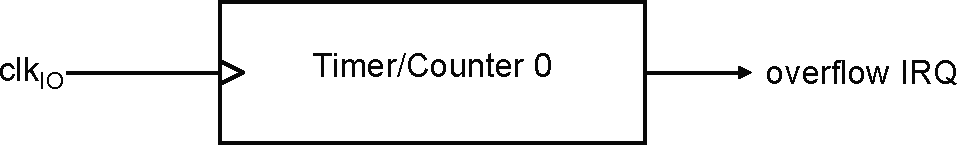
\includegraphics[scale=\figscale]{images/timsimpletc0}
\caption{Eenvoudige voorstelling van de Normal modus van Timer/Counter 0.}
\label{fig:timsimpletc0}
\end{figure}

%%%Zoals te zien is, kan in de Normal modus een interrupt gegenereerd worden als
%%%de waarde in het TCNT0-register van 255 naar 0 gaat (roll-over). Dit wordt
%%%de Timer Overflow interrupt genoemd.

Het TCNT0-register is door de gebruiker te lezen en te schrijven. Als de
software een waarde schrijft in TCNT0, dan gaat T/C0 verder tellen vanaf
deze waarde. Het is dan eenvoudig om te bepalen of de teller een bepaalde
waarde heeft. In listing~\ref{cod:waittc0} is te zien hoe TCNT0 eerst
geladen wordt met 0 en dan gewacht wordt totdat TCNT0 de waarde~123 heeft
bereikt.

\begin{figure}[!ht]
\begin{lstlisting}[language=AVRassembler,caption=Lezen van de tellerwaarde van T/C0.,label=cod:waittc0]
       ldi  r16,0        ; load TCNT0 with 0
       out  TCNT0,r16

wait:  in   r16,TCNT0    ; wait for TCNT0 to reach 123
       cpi  r16,123
       brne wait
\end{lstlisting}
\end{figure}

\subsection{Clear Timer on Compare Match Mode (CTC)}
\label{sec:tc0ctcmode}
In deze modus telt T/C0 vanaf 0 tot en met een opgegeven maximum en begint
dan weer op 0. Het opgegeven maximum wordt aangegeven door het Output Compare
Register (OCR0). Dit register moet voor aanvang van het tellen door de
gebruiker geladen worden met een waarde. Het is mogelijk om op een
\textsl{compare match} een interrupt te genereren. Een eenvoudige
voorstelling van de CTC-modus is te zien in figuur~\ref{fig:timsimplectctc0}.

\begin{figure}[!ht]
\centering
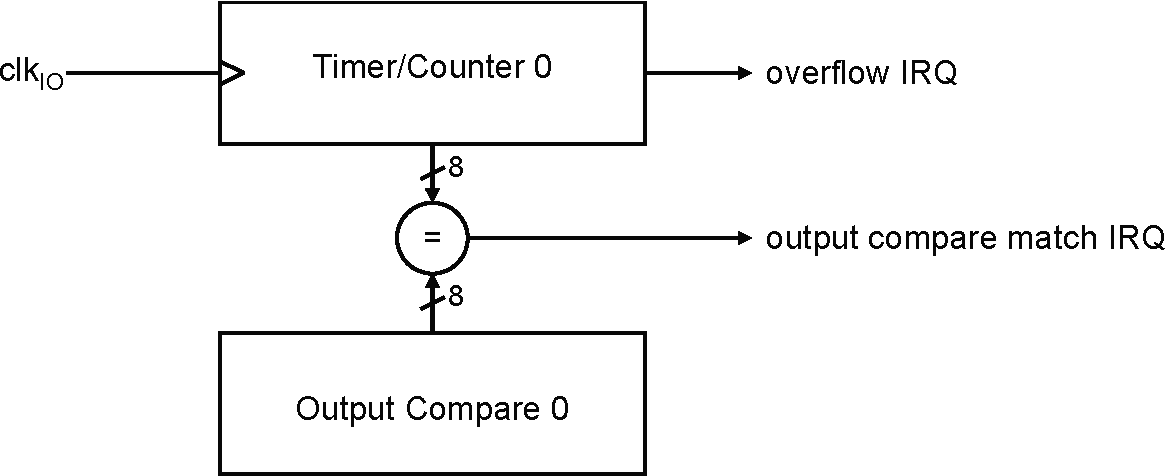
\includegraphics[scale=\figscale]{images/timsimplectctc0}
\caption{Eenvoudige voorstelling van de CTC-modus van Timer/Counter 0.}
\label{fig:timsimplectctc0}
\end{figure}

Zoals te zien is, kan in de CTC-modus een interrupt gegenereerd worden als
de waarde in het TCNT0-register en OCR0-register gelijk zijn. Dit wordt
de Output Compare Match interrupt genoemd. Merk op dat de interrupt pas
gegenereerd wordt als TCNT0 weer op~0 staat.

In listing~\ref{cod:setupocr0tc0} is te zien hoe het OCR0-register wordt
ingesteld op de waarde 143. Tevens wordt de CTC-modus geselecteerd in het
TCCR0-register. Merk op dat de teller na 144 klokpulsen weer op 0 staat.
De teller telt immers van 0 t/m 143.

\begin{figure}[!ht]
\begin{lstlisting}[language=AVRassembler,caption=Instellen van het OCR0-register van T/C0,label=cod:setupocr0tc0]
       ldi  r16,143          ; load OCR0 with 143
       out  OCR0,r16
       
       ldi  r16,0b00001000   ; select CTC mode 
       out  TCCR0,r16
\end{lstlisting}
\end{figure}

\subsection{Klokbronnen}
Al eerder is aangegeven dat T/C0 kan tellen op een intern kloksignaal of
op een extern kloksignaal. Aangezien de interne klokfrequentie vrij groot is
en het aantal timer-bits klein, zal T/C0 zeer snel op het maximum zitten en
genereert zodanig heel vaak een \textsl{timer overflow}. Vaak willen we de
timer overflow op een veel lagere frequentie laten plaatsvinden.
Een \textsl{prescaler} biedt dan uitkomst. Een prescaler is een digitale
schakeling die het aangeboden kloksignaal `deelt' door een getal, meestal een
macht van 2. Hierdoor telt T/C0 op een (veel) lagere frequentie. De prescaler
van T/C0 heeft vier mogelijke delers: 8, 64, 256 en 1024. Staat de prescaler
bijvoorbeeld op 1024 ingesteld dan wordt TCNT0 om de 1024 klokpulsen met
\'e\'en verhoogd. Dat betekent dat er eens in de~1024$\times$256 = 262144
klokpulsen 
een roll-over plaatsvindt.

Naast interne klokpulsen kan T/C0 ook externe klokpulsen tellen. Eigenlijk
telt TC/0 op \textsl{flanken}. Zo kan T/C0 op opgaande of neergaande flanken
tellen. Het externe kloksignaal moet worden aangeboden aan ingang T0
(pin 1 op een 40-pin PDIP). De prescaler kan niet ingeschakeld worden bij
gebruik van externe klokpulsen.

Natuurlijk kan T/C0 ook ``uit'' staan. T/C0 is dan gestopt met tellen. Dit is
de situatie direct na een reset.
Bij elkaar levert dit acht mogelijke klokbronnen op. Ook ``uit'' noemen we een
klokbron en de teller kan ook direct met de systeemklok gevoed worden. Dit
is met drie bits aan te geven. Dit zijn de CS0-bits in register TCCR0.

In figuur~\ref{fig:timsimplenormalctctc0} is een vereenvoudigde weergave
te zien van T/C0 met de klokbronselectie en normal- en CTC-modi. In
figuur~\ref{fig:timtccr0csbits} is de indeling van de CS0-bits in het
TCCR0-register te zien. De betekenis van de CS0-bits is te vinden in
tabel~\ref{tab:timklokselectie0}.

\begin{figure}[!ht]
\centering
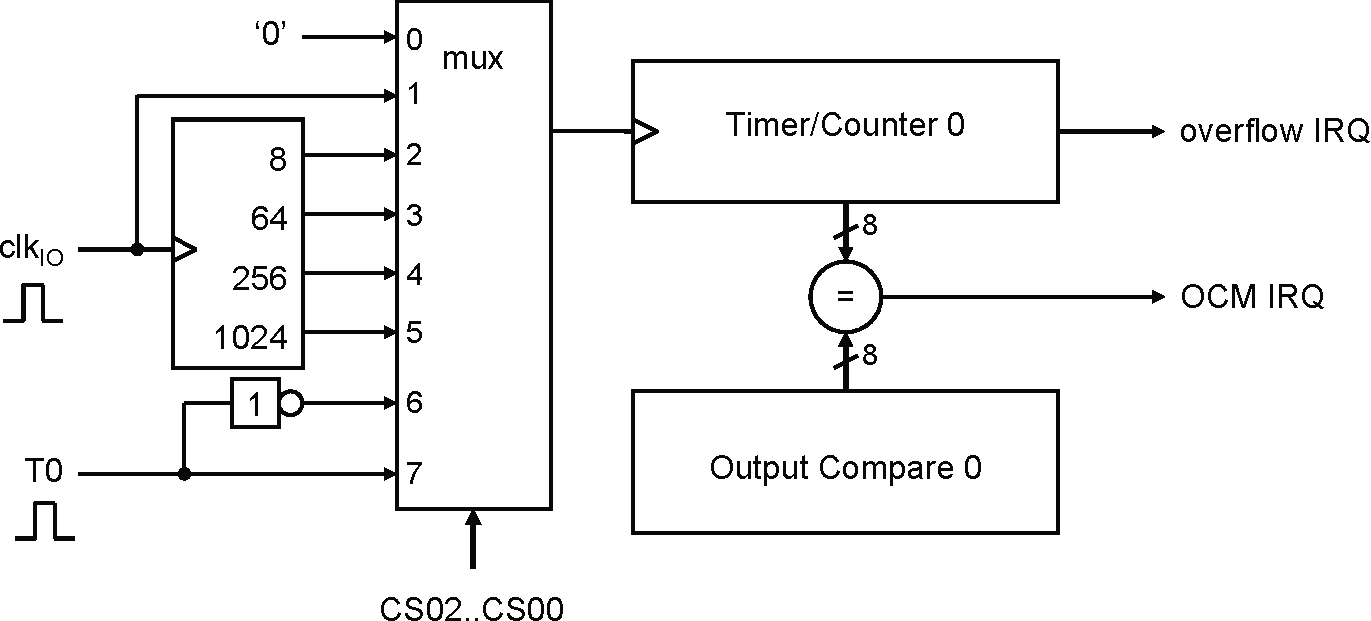
\includegraphics[scale=\figscale]{images/timsimplenormalctctc0}
\caption{Eenvoudige voorstelling van de normal en CTC-modus van Timer/Counter 0.}
\label{fig:timsimplenormalctctc0}
\end{figure}

%%%% TCCR0
\begin{registerdef}{De CS02-, CS01 en CS00-bits in het TCCR0-register}{fig:timtccr0csbits}
7 & 6 & 5 & 4 & 3 & 2 & 1 & 0 \\
\hline
\multicolumn{1}{|c}{\cellcolor{regcell} FOC0} & \multicolumn{1}{|c}{\cellcolor{regcell}WGM00} & \multicolumn{1}{|c}{\cellcolor{regcell} COM01} & \multicolumn{1}{|c}{\cellcolor{regcell} COM00} & \multicolumn{1}{|c}{\cellcolor{regcell} WGM01} & \multicolumn{1}{|c}{CS02} & \multicolumn{1}{|c}{CS01} & \multicolumn{1}{|c|}{CS00} \\ \hline
W & R/W & R/W & R/W & R/W & R/W & R/W & R/W \\
0 & 0 & 0 & 0 & 0 & 0 & 0 & 0 \\
\end{registerdef}
%%%% TCCR0

\begin{table}[!ht]
\centering
\caption{Klokbronselectie voor Timer/Counter 0.}
\label{tab:timklokselectie0}
\renewcommand\arraystretch{1.2}
%\tabulinesep=1.2mm
\begin{tabu} to 0.5\textwidth{ccc|l}
CS02 & CS01 & CS00 & operatie \\ \hline
  0  &   0  &   0  & geen werking, klok is gestopt\\
  0  &   0  &   1  & $\text{CLK}_\text{IO}/1$, geen prescaler \\
  0  &   1  &   0  & $\text{CLK}_\text{IO}/8$, van prescaler \\ 
  0  &   1  &   1  & $\text{CLK}_\text{IO}/64$, van prescaler \\
  1  &   0  &   0  & $\text{CLK}_\text{IO}/256$, van prescaler \\
  1  &   0  &   1  & $\text{CLK}_\text{IO}/1024$, van prescaler \\
  1  &   1  &   0  & externe klokbron op de T0-pin, neergaande flank \\
  1  &   1  &   1  & externe klokbron op de T0-pin, opgaande flank \\
\end{tabu}
\end{table}

De code in listing~\ref{cod:setupctcprescaler1024tc0} zorgt ervoor dat T/C0
ingesteld wordt in CTC-modus met een prescalerwaarde van 1024 als klokbron.

\begin{figure}[!ht]
\begin{lstlisting}[language=AVRassembler,caption=Selectie van CTC-modus en prescaler 1024.,label=cod:setupctcprescaler1024tc0]
       ldi  r16,0b00001101   ; select CTC mode, prescaler 1024
       out  TCCR0,r16
\end{lstlisting}
\end{figure}

\subsection{Interrupts: Timer overflow en Output Compare Match overflow}
Een taak die vaak voorkomt in de ATmega32, is het periodiek uitvoeren
van een stukje code. Te denken valt aan een temperatuurmeting die elke
minuut moet plaatsvinden. Natuurlijk kunnen we een wachtlus gebruiken,
maar de controller kan dan niets anders doen. We kunnen T/C0 gebruiken
om een stukje tijd af te meten.

In de normal-modus telt T/C0 van 0 t/m 255.
Als T/C0 een roll-over heeft, dus van telstand 255 naar telstand 0 gaat,
wordt op telstand~0 de Timer/Counter 0 Overflow Flag (TOV0) op~1 gezet.
In figuur~\ref{fig:tc0tov0} is dit grafisch uitgebeeld. Elke keer als
de teller weer op 0 staat, wordt de TOV-vlag op 1 gezet. De TOV0-vlag is
terug te vinden in het Timer/Counter Interrupt Flag Register (TIFR).

\begin{figure}[!ht]
\centering
\begin{tikzpicture}[font=\footnotesize\sffamily,>=latex,scale=1.25]
\coordinate (A) at (0,0);
\draw [ultra thick] (A) node[left] {0x00} -- ++(0,2) node[left] {0xFF};
\draw (A) -- ++(1.5,2) -- ++(0,-2) -- ++(1.5,2) -- ++(0,-2) -- ++(1.5,2) -- ++(0,-2) -- ++(1.5,2) -- ++(0,-2) -- ++(0.75,1);
\draw [ultra thick,->](A) -- (7,0) node[right] {$t$};
\draw [dashed] (0,2) -- (7,2) {};
\draw [->] (1.5,0) -- ++(-0.25,-0.75) node[below] {TOV0=1};
\draw [->] (3.0,0) -- ++(-0.25,-0.75) node[below] {TOV0=1};
\draw [->] (4.5,0) -- ++(-0.25,-0.75) node[below] {TOV0=1};
\draw [->] (6.0,0) -- ++(-0.25,-0.75) node[below] {TOV0=1};
\end{tikzpicture}
\caption{Tijddiagram van de TCNT0-waarde met de momenten van een timer overflow.}
\label{fig:tc0tov0}
\end{figure}

De TOV0-vlag is op twee manieren op 0 te krijgen: door hardware bij het
uitvoeren van een timer overflow interrupt en door software door het
schrijven van een 1 in het TIFR-register. De frequentie van de timer overflow
is te berekenen met de formule:
%
\begin{equation}
f_{ov} = \dfrac{f_{clk}}{\mathrm{prescaler}\times 256}
\end{equation}
%
Bij een frequentie van 3,6864 MHz en een prescalerwaarde van 1024 is de
overflow-frequentie dus 14,0625 Hz. Merk op dat bij deze klokfrequentie
de overflow-frequentie niet lager te realiseren is.

%%%% TIFR
\begin{registerdef}{Het TIFR-register}{fig:tc0tifr}
7 & 6 & 5 & 4 & 3 & 2 & 1 & 0 \\
\hline
\multicolumn{1}{|c}{\cellcolor{regcell} OCF2} & \multicolumn{1}{|c}{\cellcolor{regcell} TOV2} & \multicolumn{1}{|c}{\cellcolor{regcell} ICF1} & \multicolumn{1}{|c}{\cellcolor{regcell} OCF1A} & \multicolumn{1}{|c}{\cellcolor{regcell} OCF1B} & \multicolumn{1}{|c}{\cellcolor{regcell} TOV1} & \multicolumn{1}{|c}{OCF0} & \multicolumn{1}{|c|}{TOV0} \\ \hline
R/W & R/W & R/W & R/W & R/W & R/W & R/W & R/W \\
0 & 0 & 0 & 0 & 0 & 0 & 0 & 0 \\
\end{registerdef}
%%%% TIFR

\begin{figure}[!ht]
\centering
\begin{tikzpicture}[font=\footnotesize\sffamily,>=latex,scale=1.25]
\coordinate (A) at (0,0);
\draw [ultra thick] (A) node[left] {0x00} -- ++(0,2) node[left] {0xFF};
\draw (A) -- ++(1.125,1.5) -- ++(0,-1.5) -- ++(1.125,1.5) -- ++(0,-1.5) -- ++(1.125,1.5) -- ++(0,-1.5) -- ++(1.125,1.5) -- ++(0,-1.5) -- ++(1.125,1.5) -- ++(0,-1.5) -- ++(1.125,1.5) -- ++(0,-1.5) -- ++(0.5625,0.75);
\draw [ultra thick,->](A) -- (7.5,0) node[right] {$t$};
\draw [dashed] (0,2) -- (7.5,2) {};
\draw (0,1.5) node[left] {OCR0};
\draw [dashed] (0,1.5) -- (7.5,1.5) {};
\draw [->] (1.125,0) -- ++(-0.25,-0.75) node[below] {OCF0=1};
\draw [->] (2.250,0) -- ++(-0.25,-0.75) node[below] {OCF0=1};
\draw [->] (3.375,0) -- ++(-0.25,-0.75) node[below] {OCF0=1};
\draw [->] (4.500,0) -- ++(-0.25,-0.75) node[below] {OCF0=1};
\draw [->] (5.625,0) -- ++(-0.25,-0.75) node[below] {OCF0=1};
\draw [->] (6.750,0) -- ++(-0.25,-0.75) node[below] {OCF0=1};
\end{tikzpicture}
\captionsetup{width=.85\linewidth}
\caption{Tijddiagram van de TCNT0-waarde met de momenten van een output compare match overflow.}
\label{fig:}
\end{figure}














\subsection{Fast-PWM mode}
\label{sec:tc0fastpwmmode}
Volgt nog.

\subsection{Phase Correct PWM mode}
\label{sec:tc0phasecorrectpwmmode}
Volgt nog.







\section{De registers van Timer/Counter 0}
De besturing van Timer/Counter 0 is vastgelegd in het TCCR0-register, zie
figuur~\ref{fig:tccr0}. Dit register kan zowel gelezen als geschreven worden.

%%%% TCCR0
\begin{registerdef}{TCCR0 register}{fig:tccr0}
7 & 6 & 5 & 4 & 3 & 2 & 1 & 0 \\
\hline
\multicolumn{1}{|c}{FOC0} & \multicolumn{1}{|c}{WGM00} & \multicolumn{1}{|c}{COM01} & \multicolumn{1}{|c}{COM00} & \multicolumn{1}{|c}{WGM01} & \multicolumn{1}{|c}{CS02} & \multicolumn{1}{|c}{CS01} & \multicolumn{1}{|c|}{CS00} \\ \hline
W & R/W & R/W & R/W & R/W & R/W & R/W & R/W \\
0 & 0 & 0 & 0 & 0 & 0 & 0 & 0 \\
\end{registerdef}
%%%% TCCR0

\textbf{Bit 7 -- FOC0: Force Output Compare}\\
De FOC0-bit is alleen actief als we de WGM0\textsl{x}-bits non-PWM-modus specificeren. Bij
het specificeren van \'e\'en van de twee PWM-modi moet deze bit altijd als 0 geschreven
worden. Als deze bit met een 1 geladen wordt, zal de signaalvormgenerator een directe
compare match krijgen en zal de OC0-uitgang veranderen zoals is vastgelegd in de
COM0\textsl{x}-bits.

%%%The FOC0 bit is only active when the WGM00 bit specifies a non-PWM mode. However, for
%%%ensuring compatibility with future devices, this bit must be set to zero when TCCR0 is written
%%%when operating in PWM mode. When writing a logical one to the FOC0 bit, an immediate compare
%%%match is forced on the Waveform Generation unit. The OC0 output is changed according to
%%%its COM01:0 bits setting. Note that the FOC0 bit is implemented as a strobe. Therefore it is the
%%%value present in the COM01:0 bits that determines the effect of the forced compare.

\textbf{Bits 3,6 -- WGM0\textsl{x} signaalvormgeneratorbits}\\
Deze bits bepalen de telvolgorde van de Timer/Counter, de maximale telwaarde en het type
van de signaalvormgenerator. Zie tabel~\ref{tab:signaalvormgeneratie0}.

\begin{table}[!ht]
\centering
\caption{Signaalvormgeneratie}
\label{tab:signaalvormgeneratie0}
\renewcommand\arraystretch{1.2}
\begin{tabu} {cc|l|l|l|l}
WGM01 & WGM00 & Modus & Top & Update OCR0 & TOV0-vlag \\ \hline
  0   &   0   & Normaal & 255 & direct & 255 \\
  0   &   1   & Phase Correct PWM & 255 & 255 & 0 \\
  1   &   0   & CTC & OCR0 & direct & 255 \\
  1   &   1   & Fast PWM & 255 & 0 & 255
\end{tabu}
\end{table}

\textbf{Bits 5,4 -- COM0\textsl{x} Compare Match Output Mode}\\
Deze bits bepalen het gedrag van de Output Compare pin (OC0).
Merk op dat de Data Direction (DDR) bit van de OC0-pin op 1 gezet
moet worden om de uitgang te activeren.
Tabel~\ref{tab:comparematchnonpwm0} geeft de functionaliteit van
de COM0\textsl{x}-bits weer in non-PWM-modus (Normal en CTC).

\begin{table}[!ht]
\centering
\caption{Compare Match uitgang, non-PWM-modus.}
\label{tab:comparematchnonpwm0}
\renewcommand\arraystretch{1.2}
\begin{tabu} {cc|l}
COM01 & COM00 & Beschrijving \\ \hline
  0   &   0   & Normale poortwerking, OC0 is gedeactiveerd \\
  0   &   1   & Verander OC0 op een compare match (toggle) \\
  1   &   0   & Zet OC0 op 0 op een compare match \\
  1   &   1   & Zet OC0 op 1 op een compare match \\
\end{tabu}
\end{table}

Tabel~\ref{tab:comparematchfastpwm0} geeft de functionaliteit van de
COM0\textsl{x}-bits weer in Fast PWM-modus.

\begin{table}[!ht]
\centering
\caption{Compare Match uitgang, Fast PWM-modus.}
\label{tab:comparematchfastpwm0}
\renewcommand\arraystretch{1.2}
\begin{tabu} {cc|l}
COM01 & COM00 & Beschrijving \\ \hline
  0   &   0   & Normale poortwerking, OC0 is gedeactiveerd \\
  0   &   1   & Niet gebruikt \\
  1   &   0   & Zet OC0 op 0 op een compare match, zet op 1 op TCNT = 255 \\
  1   &   1   & Zet OC0 op 1 op een compare match, zet op 0 op TCNT = 255 \\
\end{tabu}
\end{table}

Tabel~\ref{tab:comparematchphasecorrectpwm0} geeft de functionaliteit van de
COM0\textsl{x}-bits weer in Phase Correct PWM-modus.

\begin{table}[!ht]
\centering
\caption{Compare Match uitgang, Fast PWM-modus.}
\label{tab:comparematchphasecorrectpwm0}
\renewcommand\arraystretch{1.2}
\begin{tabu} {cc|p{11cm}}
COM01 & COM00 & Beschrijving \\ \hline
  0   &   0   & Normale poortwerking, OC0 is gedeactiveerd \\
  0   &   1   & Niet gebruikt \\
  1   &   0   & Zet OC0 op 0 bij Compare Match bij omhoog tellen, zet OC0 op 1 bij omlaag tellen \\
  1   &   1   & Zet OC0 op 1 bij Compare Match bij omhoog tellen, zet OC0 op 0 bij omlaag tellen \\
\end{tabu}
\end{table}





\textbf{Bits 2,1,0 -- CS0\textsl{x} klokselectiebits}\\
In tabel~\ref{tab:klokselectie0} is te zien hoe een klok geselecteerd kan worden.

\begin{table}[!ht]
\centering
\caption{Klokselectie voor Timer/Counter 0.}
\label{tab:klokselectie0}
\renewcommand\arraystretch{1.2}
%\tabulinesep=1.2mm
\begin{tabu} to 0.5\textwidth{ccc|l}
CS02 & CS01 & CS00 & operatie \\ \hline
  0  &   0  &   0  & geen werking, klok is gestopt\\
  0  &   0  &   1  & $\text{CLK}_\text{IO}/1$, geen prescaler \\
  0  &   1  &   0  & $\text{CLK}_\text{IO}/8$, van prescaler \\ 
  0  &   1  &   1  & $\text{CLK}_\text{IO}/64$, van prescaler \\
  1  &   0  &   0  & $\text{CLK}_\text{IO}/256$, van prescaler \\
  1  &   0  &   1  & $\text{CLK}_\text{IO}/1024$, van prescaler \\
  1  &   1  &   0  & externe klokbron op de T0-pin, neergaande flank \\
  1  &   1  &   1  & externe klokbron op de T0-pin, opgaande flank \\
\end{tabu}
\end{table}


Het TCNT0-register is een 8-bits register en bevat de tellerwaarde van Timer/Counter~0,
zie figuur~\ref{fig:tcnt0}. Dit register kan zowel gelezen als geschreven worden. Bij
een schrijfactie telt Timer/Counter~0 verder vanaf de geschreven waarde.

%%%% TCNT0
\begin{registerdef}{Het TCNT0 register}{fig:tcnt0}
7 & 6 & 5 & 4 & 3 & 2 & 1 & 0 \\
\hline
\multicolumn{8}{|c|}{TCNT0[7:0]}  \\ \hline
R/W & R/W & R/W & R/W & R/W & R/W & R/W & R/W \\
0 & 0 & 0 & 0 & 0 & 0 & 0 & 0 \\
\end{registerdef}
%%%% TCNT0

Het OCR0-register bevat een 8-bits waarde en wordt continue vergeleken met de waarde
in het TCNT0-register, zie figuur~\ref{fig:ocr0}. Als de twee register gelijk zijn aan
elkaar kan een interrupt gegenereerd worden of kan een golfvorm gegenereerd worden op
de OC0-uitgang.

%%%% OCR0
\begin{registerdef}{Het OCR0 register}{fig:ocr0}
7 & 6 & 5 & 4 & 3 & 2 & 1 & 0 \\
\hline
\multicolumn{8}{|c|}{OCR0[7:0]}  \\ \hline
R/W & R/W & R/W & R/W & R/W & R/W & R/W & R/W \\
0 & 0 & 0 & 0 & 0 & 0 & 0 & 0 \\
\end{registerdef}
%%%% OCR0








De indeling van het TIMSK-register is te zien in figuur~\ref{fig:timsk}. Voor Timer/Counter~0
zijn alleen de bits OCIE0 (bit 1) en TOIE0 (bit 0) van belang.

%%%% TIMSK
\begin{registerdef}{Het TIMSK register}{fig:timsk}
7 & 6 & 5 & 4 & 3 & 2 & 1 & 0 \\
\hline
\multicolumn{1}{|c}{\cellcolor{regcell} OCIE2} & \multicolumn{1}{|c}{\cellcolor{regcell} TOIE2} & \multicolumn{1}{|c}{\cellcolor{regcell} TICIE1} & \multicolumn{1}{|c}{\cellcolor{regcell} OCIE1A} & \multicolumn{1}{|c}{\cellcolor{regcell} OCIE1B} & \multicolumn{1}{|c}{\cellcolor{regcell} TOIE1} & \multicolumn{1}{|c}{OCIE0} & \multicolumn{1}{|c|}{TOIE0} \\ \hline
R/W & R/W & R/W & R/W & R/W & R/W & R/W & R/W \\
0 & 0 & 0 & 0 & 0 & 0 & 0 & 0 \\
\end{registerdef}
%%%% TIMSK

\textbf{Bit 1 -- OCIE0: Timer/Counter 0 Output Compare Match Interrupt Enable} \\
Een logische 1 in deze bit zorgt ervoor dat de compare match interrupt geactiveerd wordt.
Een interrupt wordt pas daadwerkelijk uitgevoerd als de I-bit in het statusregister ook
een logische 1 is.

\textbf{Bit 0 -- TOIE0: Timer/Counter 0 Overflow Interrupt Enable} \\
Een logische 1 in deze bit zorgt ervoor dat de overflow interrupt geactiveerd wordt.
Een interrupt wordt pas daadwerkelijk uitgevoerd als de I-bit in het statusregister ook
een logische 1 is.

De indeling van het TIFR-register is te zien in figuur~\ref{fig:tifr}. Voor Timer/Counter~0
zijn alleen de bits OCF0 (bit 1) en TOV0 (bit 0) van belang.

%%%% TIFR
\begin{registerdef}{Het TIFR register}{fig:tifr}
7 & 6 & 5 & 4 & 3 & 2 & 1 & 0 \\
\hline
\multicolumn{1}{|c}{\cellcolor{regcell} OCF2} & \multicolumn{1}{|c}{\cellcolor{regcell} TOV2} & \multicolumn{1}{|c}{\cellcolor{regcell} ICF1} & \multicolumn{1}{|c}{\cellcolor{regcell} OCF1A} & \multicolumn{1}{|c}{\cellcolor{regcell} OCF1B} & \multicolumn{1}{|c}{\cellcolor{regcell} TOV1} & \multicolumn{1}{|c}{OCF0} & \multicolumn{1}{|c|}{TOV0} \\ \hline
R/W & R/W & R/W & R/W & R/W & R/W & R/W & R/W \\
0 & 0 & 0 & 0 & 0 & 0 & 0 & 0 \\
\end{registerdef}
%%%% TIFR

\textbf{Bit 1 -- OCF0: Output Compare Flag 0} \\
Deze bit wordt op een logische 1 gezet als de waarde van het OCR0-register gelijk is aan
de waarde in het TCNT0-register (compare match). Dit gebeurt op de volgende Timer/Counter
0 klokpuls. Deze bit wordt op een logische~0 gezet
als de bijbehorende interrupt wordt uitgevoerd. Als alternatief voor het op 0 zetten
kan een 1 worden geschreven naar deze bit.

\textbf{Bit 0 -- TOV0: Timer/Counter 0 Overflow Flag} \\
Deze bit wordt op een logische 1 gezet als Timer/Counter 0 een overflow veroorzaakt. Dit
gebeurt op de volgende Timer/Counter 0 klokpuls. Deze
bit wordt op 0 gezet als de bijbehorende interrupt wordt uitgevoerd. Als alternatief voor
het op 0 zetten kan een 1 worden geschreven naar deze bit. In fasecorrect PWM-modus wordt
deze bit op 1 gezet als Timer/Counter 0 van telrichting verandert op 0.

In figuur~\ref{fig:intsfior} is het SFIOR-register te zien.

%%%% SFIOR
\begin{registerdef}{Het SFIOR register}{fig:intsfior}
7 & 6 & 5 & 4 & 3 & 2 & 1 & 0 \\
\hline
\multicolumn{1}{|c}{\cellcolor{regcell} ADTS2} & \multicolumn{1}{|c}{\cellcolor{regcell} ADTS1} & \multicolumn{1}{|c}{\cellcolor{regcell} ADTS0} & \multicolumn{1}{|c}{\cellcolor{regcell} --} & \multicolumn{1}{|c}{\cellcolor{regcell} ACME} & \multicolumn{1}{|c}{\cellcolor{regcell} PUD} & \multicolumn{1}{|c}{\cellcolor{regcell}PSR2} & \multicolumn{1}{|c|}{PRS10} \\ \hline
R/W & R/W & R/W & R & R/W & R/W & R/W & R/W \\
0 & 0 & 0 & 0 & 0 & 0 & 0 & 0 \\
\end{registerdef}
%%%% SFIOR

\textbf{Bit 0 -- PRS10: Prescaler reset Timer/Counter 1 en Timer/Counter 0}\\
Wanneer deze bit met een 1 geschreven wordt, zal de prescaler van Timer/Counter 1 en
Timer/Counter 0 worden gereset. Nadat de operatie is voltooid, wordt deze bit door de
hardware op 0 gezet. Merk op dat de prescaler door zowel Timer/Counter 1 als
Timer/Counter 0 gebruikt wordt. Het beïnvloedt de werking van beide Timer/Counters.
Deze bit leest altijd als een 0.

\endinput


\end{document}